% Options for packages loaded elsewhere
\PassOptionsToPackage{unicode}{hyperref}
\PassOptionsToPackage{hyphens}{url}
\PassOptionsToPackage{dvipsnames,svgnames,x11names}{xcolor}
%
\documentclass[
  a4paper,
]{scrreprt}

\usepackage{amsmath,amssymb}
\usepackage{iftex}
\ifPDFTeX
  \usepackage[T1]{fontenc}
  \usepackage[utf8]{inputenc}
  \usepackage{textcomp} % provide euro and other symbols
\else % if luatex or xetex
  \usepackage{unicode-math}
  \defaultfontfeatures{Scale=MatchLowercase}
  \defaultfontfeatures[\rmfamily]{Ligatures=TeX,Scale=1}
\fi
\usepackage{lmodern}
\ifPDFTeX\else  
    % xetex/luatex font selection
\fi
% Use upquote if available, for straight quotes in verbatim environments
\IfFileExists{upquote.sty}{\usepackage{upquote}}{}
\IfFileExists{microtype.sty}{% use microtype if available
  \usepackage[]{microtype}
  \UseMicrotypeSet[protrusion]{basicmath} % disable protrusion for tt fonts
}{}
\usepackage{xcolor}
\setlength{\emergencystretch}{3em} % prevent overfull lines
\setcounter{secnumdepth}{2}
% Make \paragraph and \subparagraph free-standing
\ifx\paragraph\undefined\else
  \let\oldparagraph\paragraph
  \renewcommand{\paragraph}[1]{\oldparagraph{#1}\mbox{}}
\fi
\ifx\subparagraph\undefined\else
  \let\oldsubparagraph\subparagraph
  \renewcommand{\subparagraph}[1]{\oldsubparagraph{#1}\mbox{}}
\fi


\providecommand{\tightlist}{%
  \setlength{\itemsep}{0pt}\setlength{\parskip}{0pt}}\usepackage{longtable,booktabs,array}
\usepackage{calc} % for calculating minipage widths
% Correct order of tables after \paragraph or \subparagraph
\usepackage{etoolbox}
\makeatletter
\patchcmd\longtable{\par}{\if@noskipsec\mbox{}\fi\par}{}{}
\makeatother
% Allow footnotes in longtable head/foot
\IfFileExists{footnotehyper.sty}{\usepackage{footnotehyper}}{\usepackage{footnote}}
\makesavenoteenv{longtable}
\usepackage{graphicx}
\makeatletter
\def\maxwidth{\ifdim\Gin@nat@width>\linewidth\linewidth\else\Gin@nat@width\fi}
\def\maxheight{\ifdim\Gin@nat@height>\textheight\textheight\else\Gin@nat@height\fi}
\makeatother
% Scale images if necessary, so that they will not overflow the page
% margins by default, and it is still possible to overwrite the defaults
% using explicit options in \includegraphics[width, height, ...]{}
\setkeys{Gin}{width=\maxwidth,height=\maxheight,keepaspectratio}
% Set default figure placement to htbp
\makeatletter
\def\fps@figure{htbp}
\makeatother
\newlength{\cslhangindent}
\setlength{\cslhangindent}{1.5em}
\newlength{\csllabelwidth}
\setlength{\csllabelwidth}{3em}
\newlength{\cslentryspacingunit} % times entry-spacing
\setlength{\cslentryspacingunit}{\parskip}
\newenvironment{CSLReferences}[2] % #1 hanging-ident, #2 entry spacing
 {% don't indent paragraphs
  \setlength{\parindent}{0pt}
  % turn on hanging indent if param 1 is 1
  \ifodd #1
  \let\oldpar\par
  \def\par{\hangindent=\cslhangindent\oldpar}
  \fi
  % set entry spacing
  \setlength{\parskip}{#2\cslentryspacingunit}
 }%
 {}
\usepackage{calc}
\newcommand{\CSLBlock}[1]{#1\hfill\break}
\newcommand{\CSLLeftMargin}[1]{\parbox[t]{\csllabelwidth}{#1}}
\newcommand{\CSLRightInline}[1]{\parbox[t]{\linewidth - \csllabelwidth}{#1}\break}
\newcommand{\CSLIndent}[1]{\hspace{\cslhangindent}#1}

\makeatletter
\makeatother
\makeatletter
\@ifpackageloaded{bookmark}{}{\usepackage{bookmark}}
\makeatother
\makeatletter
\@ifpackageloaded{caption}{}{\usepackage{caption}}
\AtBeginDocument{%
\ifdefined\contentsname
  \renewcommand*\contentsname{Table of contents}
\else
  \newcommand\contentsname{Table of contents}
\fi
\ifdefined\listfigurename
  \renewcommand*\listfigurename{List of Figures}
\else
  \newcommand\listfigurename{List of Figures}
\fi
\ifdefined\listtablename
  \renewcommand*\listtablename{List of Tables}
\else
  \newcommand\listtablename{List of Tables}
\fi
\ifdefined\figurename
  \renewcommand*\figurename{Figure}
\else
  \newcommand\figurename{Figure}
\fi
\ifdefined\tablename
  \renewcommand*\tablename{Table}
\else
  \newcommand\tablename{Table}
\fi
}
\@ifpackageloaded{float}{}{\usepackage{float}}
\floatstyle{ruled}
\@ifundefined{c@chapter}{\newfloat{codelisting}{h}{lop}}{\newfloat{codelisting}{h}{lop}[chapter]}
\floatname{codelisting}{Listing}
\newcommand*\listoflistings{\listof{codelisting}{List of Listings}}
\makeatother
\makeatletter
\@ifpackageloaded{caption}{}{\usepackage{caption}}
\@ifpackageloaded{subcaption}{}{\usepackage{subcaption}}
\makeatother
\makeatletter
\@ifpackageloaded{tcolorbox}{}{\usepackage[skins,breakable]{tcolorbox}}
\makeatother
\makeatletter
\@ifundefined{shadecolor}{\definecolor{shadecolor}{rgb}{.97, .97, .97}}
\makeatother
\makeatletter
\makeatother
\makeatletter
\makeatother
\ifLuaTeX
  \usepackage{selnolig}  % disable illegal ligatures
\fi
\IfFileExists{bookmark.sty}{\usepackage{bookmark}}{\usepackage{hyperref}}
\IfFileExists{xurl.sty}{\usepackage{xurl}}{} % add URL line breaks if available
\urlstyle{same} % disable monospaced font for URLs
\hypersetup{
  pdftitle={Out of Control:},
  pdfauthor={Hauke Roggenkamp},
  colorlinks=true,
  linkcolor={blue},
  filecolor={Maroon},
  citecolor={Blue},
  urlcolor={Blue},
  pdfcreator={LaTeX via pandoc}}

\title{Out of Control:}
\usepackage{etoolbox}
\makeatletter
\providecommand{\subtitle}[1]{% add subtitle to \maketitle
  \apptocmd{\@title}{\par {\large #1 \par}}{}{}
}
\makeatother
\subtitle{Utilizing Implicit Data for Behavioral Science}
\author{Hauke Roggenkamp}
\date{2024-08-01}

\begin{document}
\cleardoublepage
\thispagestyle{empty}
{\centering
\hbox{}\vskip 0cm plus 1fill
{\Huge\bfseries Out of Control: \par}
\vspace{3ex}
{\Large\bfseries Utilizing Implicit Data for Behavioral Science \par}
\vspace{12ex}
{\Large\bfseries Hauke Roggenkamp \par}
\vspace{3ex}
{\Large ORCID: 0009-0005-5176-4718 \par}
\vskip 0cm plus 2fill
{\bfseries\large Research Proposal \par}
\vspace{3ex}
{\bfseries\large 2024-08-01 \par}
\vspace{12ex}
%
%
{\bfseries\large Institute of Behavioral Science and Technology \par}
\vspace{3ex}
%
{\bfseries\large University of St.~Gallen \par}
%
\vspace{12ex}
{\small Submitted in partial fulfilment of the requirements
of the degree of Doctor of Philosophy under supervision of Christian Hildebrand and Johannes Boegershausen\par}
}
\ifdefined\Shaded\renewenvironment{Shaded}{\begin{tcolorbox}[borderline west={3pt}{0pt}{shadecolor}, interior hidden, frame hidden, breakable, enhanced, boxrule=0pt, sharp corners]}{\end{tcolorbox}}\fi

\renewcommand*\contentsname{Table of contents}
{
\hypersetup{linkcolor=}
\setcounter{tocdepth}{2}
\tableofcontents
}
\bookmarksetup{startatroot}

\hypertarget{abstract}{%
\chapter*{Abstract}\label{abstract}}
\addcontentsline{toc}{chapter}{Abstract}

\markboth{Abstract}{Abstract}

Lorem ipsum dolor sit amet, consectetur adipiscing elit. Nunc malesuada
massa eget sem fringilla vehicula. Donec pulvinar diam dolor, sed
egestas sem fringilla quis. Integer vitae gravida ante. Sed mauris nisl,
luctus a mi ut, hendrerit dapibus tortor. Sed maximus consectetur metus
sit amet aliquam. Donec eu orci sit amet neque pretium euismod. Donec
egestas aliquam ex, ac dapibus nunc maximus quis. Pellentesque in
accumsan purus, dignissim interdum turpis. Etiam sed dignissim ex, quis
congue nulla. Phasellus accumsan ullamcorper leo ac iaculis. Vivamus
tempor sapien tortor, in tincidunt lorem imperdiet in. Ut convallis
imperdiet nisl at eleifend. Fusce tincidunt nunc ut metus fermentum
vestibulum. Suspendisse vel molestie arcu. Curabitur eu diam vitae
tortor placerat gravida eget ac urna. Sed quis leo a augue dapibus
aliquet ac ac metus. Mauris sit amet convallis felis, nec ullamcorper
velit. Aliquam congue est sed augue porttitor, pellentesque ullamcorper
lacus fermentum. Nunc metus mi, consectetur et est sed, vulputate
dignissim risus. Nulla et nibh lacus. Praesent commodo metus ut tellus
aliquet, ut vehicula augue elementum.

\part{INTRODUCTION}

Praesent urna magna, tincidunt at consectetur a, facilisis consequat
magna. Mauris viverra hendrerit tempus. Mauris faucibus, nisi quis
auctor volutpat, dui augue accumsan justo, ut auctor tellus augue quis
metus. Interdum et malesuada fames ac ante ipsum primis in faucibus.
Nulla et ornare tortor, non imperdiet leo. Praesent imperdiet odio arcu,
at porttitor nulla hendrerit nec. Fusce tempor mattis neque ac
elementum. Suspendisse enim dolor, scelerisque ut viverra tincidunt,
hendrerit non dolor. Etiam sagittis magna id ex maximus, vel scelerisque
nunc placerat. Phasellus ornare sapien ac justo pharetra accumsan. Sed
mollis tincidunt semper. Curabitur et iaculis dui. Interdum et malesuada
fames ac ante ipsum primis in faucibus. Vivamus a finibus purus,
consectetur interdum quam. In semper, sem in varius commodo, sapien leo
efficitur magna, rhoncus rhoncus lectus nulla sit amet lectus.

Vestibulum ut eleifend purus. Suspendisse id enim velit. Proin iaculis
maximus elit, ac tempus sem placerat ut. Mauris aliquet eget nibh sit
amet malesuada. Phasellus facilisis porta justo, nec tincidunt justo.
Nunc consectetur nibh eget quam tristique tincidunt. Sed a odio gravida,
eleifend mauris quis, sodales erat. Curabitur id magna placerat urna
aliquam commodo ac id mauris. Proin porttitor eleifend tellus at congue.
Etiam elit tellus, semper vel blandit tempor, sagittis quis risus. Ut
fringilla dui vitae elit volutpat, elementum lobortis quam scelerisque.
Duis euismod quam sit amet sollicitudin vehicula. Curabitur pulvinar leo
eu nulla aliquam gravida quis in sem. Morbi eget facilisis urna.

Ut hendrerit risus nibh. Suspendisse vehicula, lectus sit amet tincidunt
tempor, erat lacus maximus turpis, non eleifend neque massa eget ipsum.
Sed vulputate rutrum dolor nec ullamcorper. Aliquam eu risus sit amet
neque interdum placerat sit amet at nisl. Quisque ac sapien eros.
Maecenas vulputate volutpat accumsan. Vestibulum ante ipsum primis in
faucibus orci luctus et ultrices posuere cubilia curae; Nam sit amet
finibus nisl. Integer id aliquam ex. Praesent id enim sapien. Nullam
posuere tellus a arcu ullamcorper, nec bibendum mauris feugiat. Duis non
porta quam. Donec eget lectus aliquam, commodo lorem nec, auctor orci.
Fusce vitae aliquam turpis, sit amet sodales urna.

Donec eleifend cursus tellus, quis tempor arcu hendrerit tempor.
Maecenas non ornare nunc, et lacinia diam. Nulla eget nunc odio. Mauris
ultricies diam et ante dapibus, et posuere ligula auctor. Pellentesque
vel est metus. Nullam posuere maximus tincidunt. Ut varius orci ut
placerat pellentesque.

Pellentesque pretium porta ipsum, mattis sodales lacus vestibulum vitae.
Praesent eget vestibulum nibh. Ut id purus enim. Phasellus sed varius
velit. Nunc gravida orci sit amet odio bibendum varius. Sed dapibus arcu
eros, sed eleifend nisl luctus vel. Morbi gravida dignissim felis ut
posuere. Quisque dapibus convallis est, at rutrum dui tempus eget.
Aenean molestie justo in eleifend placerat. Curabitur malesuada suscipit
nulla, sit amet viverra eros rutrum eget.

\hypertarget{research-overview}{%
\chapter{Research Overview}\label{research-overview}}

Throughout this research proposal, I will refer to my research projects
either using their title or a descriptive acronym.
Table~\ref{tbl-project-overview} lists my three dissertation projects
and reports the respective authors, the title, the target journal
alongside their submission- or publication status as well as the said
acronym. Each acronym is a hyperlink that directs the interested reader
to the corresponding OSF repository. The repositories contain anonymized
raw data, code, and experimental stimuli. If not stated otherwise, we
pre-registered the sample size, predictions, analysis strategy, and
data-exclusion criteria for each study of each project.

This section outlines the projects briefly to then describe how the sum
of these projects relates to the overall goal of the dissertation. The
subsequent sections then describe the individual projects on a more
granular level.

\hypertarget{tbl-project-overview}{}
\begin{longtable}[]{@{}
  >{\raggedright\arraybackslash}p{(\columnwidth - 8\tabcolsep) * \real{0.0495}}
  >{\raggedright\arraybackslash}p{(\columnwidth - 8\tabcolsep) * \real{0.2178}}
  >{\raggedright\arraybackslash}p{(\columnwidth - 8\tabcolsep) * \real{0.4208}}
  >{\raggedright\arraybackslash}p{(\columnwidth - 8\tabcolsep) * \real{0.1931}}
  >{\raggedright\arraybackslash}p{(\columnwidth - 8\tabcolsep) * \real{0.1188}}@{}}
\caption{\label{tbl-project-overview}Project Overview}\tabularnewline
\toprule\noalign{}
\begin{minipage}[b]{\linewidth}\raggedright
Acronym/OSF
\end{minipage} & \begin{minipage}[b]{\linewidth}\raggedright
Authors
\end{minipage} & \begin{minipage}[b]{\linewidth}\raggedright
Title
\end{minipage} & \begin{minipage}[b]{\linewidth}\raggedright
Target Journal
\end{minipage} & \begin{minipage}[b]{\linewidth}\raggedright
Status
\end{minipage} \\
\midrule\noalign{}
\endfirsthead
\toprule\noalign{}
\begin{minipage}[b]{\linewidth}\raggedright
Acronym/OSF
\end{minipage} & \begin{minipage}[b]{\linewidth}\raggedright
Authors
\end{minipage} & \begin{minipage}[b]{\linewidth}\raggedright
Title
\end{minipage} & \begin{minipage}[b]{\linewidth}\raggedright
Target Journal
\end{minipage} & \begin{minipage}[b]{\linewidth}\raggedright
Status
\end{minipage} \\
\midrule\noalign{}
\endhead
\bottomrule\noalign{}
\endlastfoot
\href{https://osf.io/jcxvk/}{DICE} & Roggenkamp, Boegershausen \&
Hildebrand & Digital In-Context Experiments (DICE): Enhancing Ecological
Validity and Causal Inference in Social Media Research & Journal of
Marketing & RR \\
\href{https://osf.io/jcxvk/}{CIVILITY} & Roggenkamp & The Price of
Civility: Economic and Social Returns on Investment in Toxicity
Moderation & Marketing Letters & \\
\href{https://osf.io/qswrz/}{SOUND} & Gaerth, Roggenkamp \& Hildebrand &
The Sound of Certainty: Assessing Paralinguistic Indicators of Decision
Confidence & Journal of Marketing Research & \\
\end{longtable}

\part{INDIVIDUAL PROJECTS}

Maecenas vehicula vestibulum dolor, sit amet pellentesque lacus sagittis
at. Duis elit elit, iaculis sit amet magna eget, elementum iaculis ante.
Fusce ultricies felis non ornare gravida. Praesent tempor bibendum augue
sit amet porta. Nam aliquam auctor lectus vitae rhoncus. Donec eget
tortor purus. Cras bibendum lacinia tortor. Aliquam erat volutpat. Donec
efficitur tempus tellus, iaculis ultricies tellus posuere ac.
Pellentesque ut placerat mi. Interdum et malesuada fames ac ante ipsum
primis in faucibus. Pellentesque habitant morbi tristique senectus et
netus et malesuada fames ac turpis egestas. Nam at auctor sapien.

Maecenas metus tellus, blandit at venenatis at, consectetur vitae
tellus. Nunc nec feugiat metus. Nulla nec iaculis dui. Vestibulum
pretium ullamcorper pharetra. Nullam vehicula nibh in nunc fermentum
sollicitudin. Phasellus massa erat, finibus at turpis a, aliquet tempor
metus. In hac habitasse platea dictumst. In eros lorem, sodales id nisl
vitae, lacinia mollis dui. Vivamus mollis vel libero quis malesuada.
Pellentesque viverra blandit faucibus. Mauris posuere sodales nisl vel
ullamcorper.

Sed imperdiet lectus id est malesuada consectetur. Suspendisse et elit
sed ante porta egestas a rhoncus nulla. Mauris quis ex quam. Morbi nec
porta odio. Aliquam sit amet elit vel est egestas ultrices vel malesuada
arcu. Cras vitae urna in ipsum iaculis vestibulum sit amet vel nulla.
Nam imperdiet tristique tincidunt. Donec nec mauris erat. Morbi blandit
nulla ante, id posuere nisi gravida vitae. Mauris odio mi, vulputate a
mattis in, posuere sit amet nisi. Morbi id nisi vel turpis efficitur
ultrices vel vitae dolor. Morbi a facilisis erat, facilisis malesuada
velit. Sed lacinia bibendum enim, eu molestie est euismod in. Praesent
in est at dolor bibendum laoreet. Morbi ullamcorper nisi et pellentesque
venenatis.

Nullam rutrum id felis a euismod. Nam ac risus in nisi congue commodo.
Donec placerat lobortis enim id viverra. Ut venenatis augue magna, eu
cursus mauris ultrices nec. Nulla vel dui vitae diam mattis ullamcorper.
Vestibulum ante ipsum primis in faucibus orci luctus et ultrices posuere
cubilia curae; Etiam iaculis dapibus orci ut semper. Donec sagittis
risus nunc, quis egestas est tempor non. Sed condimentum finibus mattis.

\hypertarget{digital-in-context-experiments-dice}{%
\chapter{Digital In-Context Experiments
(DICE)}\label{digital-in-context-experiments-dice}}

Co-authored with Johannes Boegershausen (Rotterdam School of Management)
and Christian Hildebrand (University of St.~Gallen), we are finalizing
the data collection and the manuscript for a re-submission at the
Journal of Marketing's special issue on
\href{https://www.ama.org/journal-of-marketing-call-for-papers-marketing-impact-with-research-driven-apps/}{\emph{``Marketing
Impact with Research-Driven Apps''}}.

\hypertarget{introduction-1}{%
\section{Introduction}\label{introduction-1}}

With 4.76 billion social media users in 2023 (i.e., approximately 60\%
of the world's population) and an average daily social media usage of
more than 2.5 hours (Kemp 2023), understanding the consequences of
social media use carries tremendous economic and societal weight (e.g.,
Ahmad et al. 2024; Anderson and Wood 2021; M. Appel, Marker, and Gnambs
2020; Orben and Przybylski 2019; Stephen 2016). Consequently, the last
two decades have seen an explosive growth of research examining consumer
and firm behavior on social media platforms (for recent reviews, see
Aridor et al. 2024; Leung, Gu, and Palmatier 2022; Shankar et al. 2022;
G. Appel et al. 2020). Consumer attention and engagement on social media
platforms have become key assets in the digital (attention) economy,
driving billion-dollar valuations of companies and leading to major
investments by brands to harness these platforms effectively.

To better understand attention and engagement on social media,
researchers strive to get access to proprietary data directly from these
platforms as they own granular data that is less susceptible to
selection issues such as algorithmic interference Xu, Zhang, and Zhou
(2020) than what is publicly available. However, most researchers do not
have the option of using confidential data because platforms are
hesitant to share these data (due to perceived regulatory, legal, or
competitive risk). Even when platforms provide data another challenge
may arise because researchers may be limited to studying topics that
could benefit the company, or, at the very least, will not hurt it
(Farronato, Fradkin, and Karr 2024, 4).

To address these challenges and to provide researchers with an
accessible method for studying social media behavior, this paper
introduces Digital-In-Context-Experiments (DICE). DICE is an open-source
tool that allows researchers to mimic and manipulate social media feeds
and track study participants' interactions with that feed, offering a
novel approach to understanding user behavior on social media platforms.
This method complements and extends existing research paradigms in our
field, which has primarily employed four approaches: scenario-based
vignette studies, observational social media studies, online platform
studies, and browser extensions.

Scenario-based vignette studies typically use a set of static vignettes
(e.g., an image or screenshot of a single or a few selected Twitter
posts) and are the back bone of consumer research. They offer high
levels of internal validity, yet they can be criticized for being too
artificial (Morales, Amir, and Lee 2017). In online platform studies
researchers can use social media platforms as hidden recruitment tools
and disguise their stimuli as ads that are displayed to the social media
platforms' real user base. Importantly, researchers can make use of
``A/B testing'' functionalities and expose different variants of the ads
to different users. However, this approach scores low on internal
validity because, unlike in experiments, the assignment of users to
these ad variants is affected by a platform's algorithms (Braun et al.
2024) and thus, not random. Observational study designs are yet another,
non-experimental approach to study social media. They leverage
proprietary datasets, web scraping, or application programming
interfaces (API) to capture archival data from social media platforms
(Boegershausen et al. 2022). While such data captures actual behavior,
these gains in realism typically come at the expense of construct
validity, internal validity, and endogeneity issues. Jointly, these
factors exacerbate the detection of causal effects and require
sophisticated econometric modeling approaches (Goldfarb, Tucker, and
Wang 2022) as well as natural experiments. However, these are
challenging to find, provide information about only specific causal
effects, and involve assumptions that are difficult to validate
empirically (Grosz et al. 2024). Hence, researchers in neighboring
disciplines have started to use custom software (i.e., browser
extensions) to conduct experiments. Under this paradigm, recruited
participants install software which can implement interventions while
tracking consumer behavior online (see, e.g., Farronato, Fradkin, and
Karr 2024; Aridor 2024; Allcott, Gentzkow, and Song 2022). Whereas this
approach offers experimentation in realistic environments as well as
stable and random group assignment, it usually requires software
development making it inaccessible for many researchers. In fact, to the
best of our knowledge, there are no published studies in the field of
marketing using this paradigm to date.

In summary, \emph{accessible} approaches to derive causal inference in
realistic social media settings remain limited and, none of them
captures the actual context of social media experiences: vignette
studies intentionally neglect contextual factors, platform studies do
allow the manipulation of contexts and do not report contextual data
whereas observational studies' archival data can capture these data but
may be affected by algorithmic interference. Consequently, researchers
are often unable to fully control, manipulate, or even observe the
contextual factors that have been shown to affect consumer behavior
(see, e.g., study 3 in Berger and Milkman 2012; or Schmitt 1994).
Furthermore, none of the approaches reports granular data that describe
individual browsing behavior. Instead, vignette studies often elicit
self-reports whereas platform- and observational data provide behavioral
data such as clicks or likes on an aggregate level. Whereas these data
are important to inform (conscious) psychological processes and
ecologically valid behavior, they tend to miss out on unconscious and
passive user behavior, that is, internal processes that do not translate
into mouse clicks (Baumeister, Vohs, and Funder 2007).

DICE addresses these limitations by making three key contributions.
First, it maintains the high internal validity characteristic of static
scenario-based vignette studies while enhancing ecological validity by
creating interactive stimuli in realistic look-and-feels. Second, it
provides researchers with control over context that also allows them to
create interventions that manipulate it. This essentially enables them
to systematically vary individual social media posts or even complete
social media feeds to examine how different (contextual) factors
influence user behavior. Third, it enables unobtrusive tracking of
implicit behavioral data, measuring the duration and timing of a
participant's interaction with each social media post. This provides
metrics that are highly used by platforms internally (see, e.g., Berger,
Moe, and Schweidel 2023; Cramer 2015; Yi et al. 2014) but unavailable
through any accessible research paradigm.

\texttt{{[}Taken\ together,\ DICE\ provides\ a\ tool\ to\ work\ on\ research\ questions\ that\ couldn\textquotesingle{}t\ be\ answered\ before...\ and\ in\ a\ way\ that\ was\ not\ accessible\ before.{]}}

We developed DICE with the aim to complement (and not replace) existing
research paradigms---static scenario-based vignette studies,
observational studies, and online platform studies. We also designed it
to be useful to a broad range of marketing stakeholders, such as brand
managers, influencers, agencies, and policy makers---with and without
programming experience. For this reason, the software consists of two
components. At its core, DICE is an oTree app (Chen, Schonger, and
Wickens 2016) that can be extended and customized by stakeholders
\emph{with} basic programming experience. In addition, we created a web
interface (\href{https://www.dice-app.org/}{www.dice-app.org}) designed
for stakeholders \emph{without} programming experience. To further
increase its ease of use, we designed DICE as a module that can be
embedded in the experimentalists' typical workflow as it is compatible
with recruitment procedures in behavioral labs or Prolific and survey
tools such as Qualtrics.

While developing DICE, we applied principles of the Open Science
movement to make research software widely available, interoperable, and
reusable. We hope that by leveraging oTree, which is frequently used in
incentive-compatible group experiments but, admittedly, not yet
established in marketing research, other researchers can add to DICE's
functionalities. For instance, to adapt media platform or to mimic the
interface of the social also mimic mass media feeds, product review
platforms or web shops.

In what follows, we first provide a critical synthesis of the three
dominant research paradigms employed in extant social media research and
their implications for validity (see Table 1) to derive our first
contribution: the enhancement of ecological validity while maintaining
high internal validity. Next, we introduce DICE, its configuration,
workflow, integration with existing research tools, participant and data
management, and its novel behavioral tracking capabilities.
Subsequently, we present two case studies that further illustrate the
workflow and the obtained data. Importantly, these studies showcase how
to leverage the control over context as well as the implicit behavioral
data, supporting our second and third contributions respectively. The
first case study demonstrates how DICE allows for precise manipulation
of social media contexts, enabling researchers to examine the impact of
varying environmental factors on user behavior. The second case study
highlights DICE's capacity to capture fine-grained behavioral metrics,
such as dwell time and scrolling patterns, providing insights
unavailable through traditional methods. Finally, we conclude with a
roadmap on how DICE might be leveraged to shape future social media
research and offer directions for key stakeholders in the social media
ecosystem (e.g., brands, influencers, and public policy).

\hypertarget{research-paradigms-in-social-media-research}{%
\section{Research paradigms in social media
research}\label{research-paradigms-in-social-media-research}}

This section also discuss the implications of these paradigms for
construct validity, internal validity, and ecological validity given
their critical role for the quality of the inferences made in marketing
research and are critical during the review process at top marketing
journals (Jacoby 1978; J. G. Lynch, Osselaer, and Torres 2024; Sridhar
et al. 2022). Construct validity, with its focus on the validity of
inferences about higher order constructs, and internal validity, with
its focus on the validity of causal relationships (Shadish, Cook, and
Campbell 2002; Xu, Zhang, and Zhou 2020), are often considered necessary
but not sufficient for high-quality marketing research (e.g., Schmitt et
al. 2022; Heerde et al. 2021). Specifically, scholars continue to call
for greater realism and external validity in marketing research (e.g.,
Jedidi et al. 2021; Morales, Amir, and Lee 2017; Jr. Lynch John G.
1982). External validity concerns whether the cause-effect relationship
holds over variations in study design, setting, samples, and measurement
variables (@ Shadish, Cook, and Campbell 2002). Because every result is
valid to some setting and no result is externally valid to all settings,
we focus our discussion to the related, yet distinct concept of
ecological validity. It refers to the extent to which research findings
can be generalized to real-life settings. It focuses on how closely the
study's methods, materials, and setting approximate the real-world
situation under investigation. High ecological validity means the
study's conditions are similar to those in the real world, making the
results more likely to be applicable in natural contexts. When deciding
between different research paradigms, scholars often face a trade-off
between different types of validity, as we will detail in the following.

\texttt{{[}Limit\ Scope\ and\ mention\ that\ real\ RCTs\ are\ impossible\ without\ the\ platforms\textquotesingle{}\ data\ and\ that\ browser\ extensions\ are\ equally\ inaccessible.{]}}

\hypertarget{scenario-based-vignette-studies}{%
\subsection{Scenario-based vignette
studies}\label{scenario-based-vignette-studies}}

Scenario-based vignette studies typically feature an image of a single
social media post that varies the focal construct(s) of interest between
different experimental conditions. For example, participants in Study 2
of Zhou, Du, and Cutright (2022, see Web Appendix F for the stimuli)
were randomly shown one of two images displaying only a single tweet
ostensibly from the brand KitKat. The image of the tweet either praised
a competitor or featured a control message. Subsequently, study
participants reported their attitudes toward both Kit Kat and a
competitor brand (i.e., Twix).\footnote{The authors used three
  seven-point scales (i.e., ``negative/positive''
  ``dislikeable/likeable'' and ``unfavorable/favorable'').} Among the
three accessible paradigms of social media studies, scenario-based
vignettes offer the highest level of internal validity as researchers
have full control over the treatment (e.g., experimental manipulations),
measurement of variables, and the randomization process. By carefully
designing their stimuli and measures, researchers can also achieve high
levels of construct validity (i.e., close alignment between the specific
operationalization and the higher-order theoretical construct). These
studies are generally easy to design, execute, and analyze.

However, experiments with static vignettes are often criticized for
their low levels of ecological validity (Morales, Amir, and Lee 2017)
and as ``research-by-convenience'' (Ferber 1977; Baumeister, Vohs, and
Funder 2007) failing to sufficiently mimic an environment that would be
informative of consumers' actual responses observable in a real
consumption setting. Static vignette studies also magnify the salience
of the focal aspects of the treatment (e.g., a particular post from a
brand), which increases the risk of demand effects and may overestimate
the size of the observed effect compared to a more noisy field setting
(see, e.g., Simonsohn, Montealegre, and Evangelidis 2024)
\texttt{(e.g.,\ Dubois\ et\ al.\ 2021)}.

A particular concern for social media research is that the prototypical
vignette social media study lacks the rich context of the actual user
experience on social media sites. Rather than seeing a single post,
consumers browse endless feeds in which many posts compete for their
attention and engagement. Thus, static vignette studies may lead
participants to adopt overly analytical mindsets that diverge from how
they would approach the same post while browsing social media platforms
(see, e.g., Pham (2013)'s 6th sin of consumer psychology).

\texttt{{[}Also\ mention\ that\ this\ focus\ on\ single\ posts\ limits\ the\ research\ questions\ on\ can\ answer.{]}}

\hypertarget{online-platform-studies}{%
\subsection{Online platform studies}\label{online-platform-studies}}

Given these limitations online platform studies have emerged as an
increasingly popular third paradigm in social media research. Since
2021, more than thirty articles in the leading marketing journals have
used such study designs (Cornil et al. 2023). Specifically, researchers
use the A/B testing functionalities provided by social media platforms,
such as Meta (i.e., Facebook and Instagram), Twitter, or LinkedIn to
compare the effect of different ads in a naturalistic social media
environment (Braun et al. 2024). The A/B testing functionalities offered
by these platforms are primarily intended for advertisers, fairly easy
to use, and provide an opportunity to study consumer behaviors in the
wild by tracking conversion outcomes across the purchase funnel such as
impressions, clicks \texttt{{[}or\ likes\ and\ comments?{]}}.

Another benefit of these online platform studies is that online ad
platforms provide some functionalities to target users based on
demographics or ``user interests'' based on their past online behavior
(Cornil et al. 2023). For example, in Study 1 of Zhou, Du, and Cutright
(2022), 13,719 Facebook users saw an ad for the Facebook page of a
fictional car wash provider. The authors use three different ads
featuring either a self-promotion, an external endorsement, or a
brand-to-brand praise message from the car wash company. Like other
online platform studies, Zhou, Du, and Cutright (2022) leverage the
aggregate summary statistics (i.e., clicks/impressions) provided by
Facebook to compute and compare the clickthrough rates of these three
different ad creatives. Online platform studies promise higher
ecological validity as they excel in realism and naturalism, given that
they are conducted directly on social media sites used by major
advertisers, while still allowing researchers (limited) control of the
stimuli and the users exposed to the stimuli.

While the A/B testing functionalities of social media platforms might
appear to be randomized controlled trials (RCTs) run in a naturalistic
environment. If they were indeed RCTs, online platform studies would be
the gold standard in social media research. Yet, by using the A/B
testing functionalities provided by digital platforms, researchers
relinquish control over critical elements of the study design to the
digital platform. Specifically, online platforms employ
post-randomization targeting algorithms that prevent clean random
assignment of participants to different treatments. Researchers' stimuli
(i.e., ads) compete in a bidding system in the digital advertising
marketplace, producing a so-called ``divergent delivery'' across
different ads (i.e., conditions) that emerges as the platform selects
users based on expected audience reaction and bid amount (Braun and
Schwartz 2023; Johnson 2023).

Additionally, at any given point in time, social media platforms are
likely to run numerous A/B tests of their own to optimize their platform
that are unobservable to researchers and may comingle with their study.
These concerns about construct validity and internal validity severely
limit the quality of inferences from these studies (see also Gordon,
Moakler, and Zettelmeyer 2022). Unfortunately, many social media
platforms like Meta do not present the mechanisms underlying these types
of studies (i.e., so-called split or A/B tests) and their limitation
very transparently (Langhe and Puntoni 2021).

Another limitation of online platform studies is that they only provide
aggregate data. While the summary data of clicks and impressions allows
researchers to generate datasets for analysis, it prevents any serious
individual-level analysis of the psychological processes driving
consumer responses (e.g., clicking sequence, time spent on a post). At
present, and despite their increasing popularity in marketing research,
it is unclear whether online platform studies have sufficient levels of
internal and construct validity to be informative for academic research
at all Braun and Schwartz (2023). Yet, it is already clear that online
platform studies are not a panacea to offset the limited realism of
typical static scenario-based vignette studies.

\texttt{{[}Make\ clear\ that\ online\ platform\ studies\ are\ not\ necessarily\ social\ media\ studies.\ Often\ they\ just\ use\ social\ media\ as\ a\ recruitment\ platform\ that\ is\ unnoticed\ by\ its\ participants.\ Many\ online\ platform\ studies\ are\ as\ much\ about\ social\ media\ as\ prolific\ studies\ are\ about\ online\ behavior.\ Just\ because\ someone\ is\ recruited\ in\ an\ social\ media\ or\ online\ environment,\ it\ does\ not\ mean\ that\ one\ studies\ behavior\ in\ there.{]}}

\hypertarget{observational-social-media-studies}{%
\subsection{Observational social media
studies}\label{observational-social-media-studies}}

A third, non-experimental paradigm, observational social media studies,
directly accesses existing social media data. Typically, researchers
collect such datasets themselves via web scraping or application
programming interfaces (Boegershausen et al. 2022), or purchase them
from proprietary sources (e.g., social media agencies in Wies, Bleier,
and Edeling 2023). Various social media sites such as Twitter (\#2, N =
27) and Facebook (\#6, N = 13) are among the most frequently scraped
sources in articles published in the leading marketing journals
(Boegershausen et al. 2022). An example of such an observational social
media study is the pilot study of Zhou, Du, and Cutright (2022),
featuring 8,393 tweets from three gaming console manufacturers between
September 1st, 2016 to September 30th, 2017 collected via the Twitter
API. The authors coded the tweets for their focal construct of interest
(i.e., whether they mentioned a competitor) and compared aggregate user
reactions to the different types of tweets (i.e., number of likes,
number of retweets). A critical advantage of such observational data is
that it features consequential dependent variables (e.g., likes,
comments, and retweets/reshares) of interest to marketing managers,
content creators, and other decision-makers (Inman et al. 2018). As
researchers can collect such data unobtrusively, these studies are
unlikely to be affected by demand effects and help identify ecologically
valid effects ``in the real world''.

Yet, observational studies are likely affected by ``algorithmic
interference'' (Boegershausen et al. 2022), which is the effect of
personalization algorithms on information display and retrieval (Xu,
Zhang, and Zhou 2020). This interference occurs both during the data
generation stage (e.g., which tweets users are exposed to) and the data
retrieval stage (e.g., which tweets researchers can retrieve). These
concerns are particularly pronounced for social media research that
draws from online platforms heavily relying on sophisticated, dynamic,
black-box algorithms (Aridor et al. 2024). The opaqueness and lack of
control over these algorithms that shape the data-generating process on
social media platforms make it difficult to address these concerns,
reducing construct and internal validity in observational social media
studies (e.g., Davidson et al. 2023; Xu, Zhang, and Zhou 2020).

Because observational social media studies are based on archival data,
researcher cannot intervene to exogenously manipulate treatment
variables. Hence, these datasets require careful consideration of the
familiar methodological challenges encountered with organically
generated data, due to potential as endogeneity issues (see, e.g., Rutz
and Watson (2019); Goldfarb, Tucker, and Wang (2022)). To overcome these
challenges, researchers typically exploit natural experiments in which
the assignment of treatments to users is ``as good as random'' (Angrist
and Pischke 2009) because it is chosen by nature or policy rather than
an experimenters. They then and apply regression discontinuity,
difference-in-differences as well as instrumental variable designs to
these natural experiments to identify causal effects. However, natural
experiments are rare to find and the corresponding methods involve
postulates, that is, assumptions that are difficult to validate
empirically (Grosz et al. 2024).

Finally, given the increased privacy regulations in the EU and other
major markets, most observational studies only contain limited
individual-level data and data granularity to explore the psychological
processes producing consumer reactions to content.

\hypertarget{app-implementation}{%
\section{App Implementation}\label{app-implementation}}

\begin{quote}
\emph{Submissions to the special issue should include a new section
titled ``App Implementation.'' In this section, the author(s) should:
(1) Describe the problem solved by the app and how it supplements the
research contribution of the manuscript. (2) Define the audience or the
end users targeted by the app and the usefulness of the app to this
audience over and above the current situation or available (software or
other) solutions. The audience can be broad and include managers,
executives, researchers, consumers, policy makers, government, media,
general public, other marketing academics, and students. (3) Provide a
secure, anonymous relatively permanent link to the app, with appropriate
instructions on how to use the app and interpret the results. Share
open-source access to the app to allow accelerated dissemination upon
publication.}
\end{quote}

\begin{quote}
\emph{Ideally, the app implementation informs the problem statement and
intended contribution of the research and manuscript.}
\end{quote}

\hypertarget{sec-dice-case-studies}{%
\section{Case Studies}\label{sec-dice-case-studies}}

The following case studies demonstrate the practical application and
novel capabilities of DICE. They not only showcase the tool in action
but also highlight its key contributions, particularly by manipulating
entire feed contexts and in measuring dwell time. By presenting these
studies, we aim to provide a blueprint for researchers interested in
adopting DICE for their own studies The first case study illustrates the
tool's capacity for manipulating and controlling entire feed contexts
whereas the second focuses on measuring participant engagement through
dwell times. Together, these studies exemplify how our tool can enhance
ecological validity while maintaining high levels of internal validity
as discussed above.

\hypertarget{context-case}{%
\subsection{Context Case}\label{context-case}}

Brand safety refers to strategies and measures ensuring that a brand's
content, particularly advertisements, does not appear in contexts that
could harm the brand's reputation (e.g., Bellman et al. 2018; Lee, Kim,
and Lim 2021; Hemmings 2021). These measures are especially crucial in
social media, where platforms use automated systems to place ads in
dynamic, rapidly changing, and user-generated content environments.
These automated systems often lack the nuanced understanding that humans
possess, potentially leading to ad placements in contexts that are only
superficially fitting but, ultimately, inappropriate.

In our hyper-connected world, such of misplacement can rapidly
propagate, potentially magnifying reputational damage beyond the initial
exposure (Swaminathan et al. 2020). Accordingly, Ahmad et al. (2024)
found that most brand managers have a strong preference to avoid
misplacement (and also that most of them are unaware that their
companies' advertising appears on misinformation websites).

To illustrate the unique capabilities of DICE, we propose a simple study
that extends beyond altering individual posts to modifying entire feeds:
Unlike traditional online platform studies, we hold the ad copy and
creative constant while manipulating the surrounding context
between-subjects. Doing so, we test the intuitive hypothesis that an
inappropriate (compared to a generic) context negatively affects brand
attitudes. To better understand whether the effect is also driven by
implicit memory effects (Schmitt 1994), we also control for aided and
unaided recall.

\hypertarget{experimental-design}{%
\subsubsection{Experimental Design}\label{experimental-design}}

We simulated a scenario where an airline inadvertently promotes a travel
destination recently impacted by a natural disaster.\footnote{This
  approach mirrors real-world practices; for instance, the German
  airline Lufthansa actively monitors news coverage and maintains a
  blacklist of affected travel destinations to avoid such misplacements.}
More specifically, we exposed participants in the treatment group to a
simulated Twitter feed that consisted of real tweets describing the
\href{https://www.bbc.com/news/articles/cle07g0zzqeo}{severe flooding}
affecting Brazil in 2024. Within this feed, we included a fictitious
sponsored post by KLM, advertising flights to Brazil with the following
copy:

\begin{quote}
Brazil's wild beauty calls! Experience nature like never before. Book
your breathtaking adventure with KLM.
\end{quote}

\texttt{{[}Add\ creative\ saying\ "Brazil.\ Wild\ Beauty.\ Book\ flight.{]}}

In contrast, the control group was exposed to the same ad but in a
different context which did not contain any tweets covering the
flooding.\footnote{You can browse the flooding-related feed
  \href{https://web.archive.org/web/20240509200732/https://ibt-hsg.herokuapp.com/p/6ni2o3bv/DICE/C_Feed/3}{here}
  and the more general feed
  \href{https://web.archive.org/web/20240509200758/https://ibt-hsg.herokuapp.com/p/97fable0/DICE/C_Feed/3}{here.}}
Instead, the control condition's feed covered other real topics such as
\emph{Madonna}'s free concert that was attended by 1.6 million people in
Rio de Janeiro at that time.

\textbf{Procedure and Measures:}
\texttt{{[}Describe\ procedure\ briefly.{]}} After participants were
exposed to their assigned social media feed, they evaluated the target
brand (KLM) on three seven-point scales presented in a random order (1 =
``Negative/Unfavorable/Dislike'' and 7 = ``Positive/Favorable/Like''),
which we average into a single measure.
\texttt{{[}We\ also\ measure\ recall.{]}}

\textbf{Participants:} We recruited 299 participants (\(M_{age} = 37\)
years; 49\% female) from the US using Qualtrics and randomly assigned
them to one of two conditions ``safe'', i.e., general feed content,
vs.~``unsafe'', i.e., flooding-related content in a between-subjects
design. All participants who started the experiment and read the
instructions (N=317), submitted the social media feed. 299 finished the
qualtrics survey. Of these 299 participants, 111 have been assigned to
the unsafe condition, specifically, the misplaced advertisement. The
subsequent table demonstrates that the two treatment groups do not
exhibit significant differences in observables. Nevertheless, the unsafe
condition tends to skew slightly younger, as indicated by column 2 in
Table~\ref{tbl-balance}. Moreover, we do not observe selective attrition
and are confident that the group assignment was indeed random---an
assumption that is generally accepted in vignette studies, but cannot be
presumed in observational studies.

\hypertarget{tbl-balance}{}
\begin{longtable}[]{@{}
  >{\raggedright\arraybackslash}p{(\columnwidth - 12\tabcolsep) * \real{0.2111}}
  >{\centering\arraybackslash}p{(\columnwidth - 12\tabcolsep) * \real{0.1111}}
  >{\centering\arraybackslash}p{(\columnwidth - 12\tabcolsep) * \real{0.1444}}
  >{\centering\arraybackslash}p{(\columnwidth - 12\tabcolsep) * \real{0.1444}}
  >{\centering\arraybackslash}p{(\columnwidth - 12\tabcolsep) * \real{0.1111}}
  >{\centering\arraybackslash}p{(\columnwidth - 12\tabcolsep) * \real{0.1333}}
  >{\centering\arraybackslash}p{(\columnwidth - 12\tabcolsep) * \real{0.1444}}@{}}
\caption{\label{tbl-balance}Balance Across Conditions}\tabularnewline
\toprule\noalign{}
\begin{minipage}[b]{\linewidth}\raggedright
\textbf{Characteristic}
\end{minipage} & \begin{minipage}[b]{\linewidth}\centering
\textbf{Beta}
\end{minipage} & \begin{minipage}[b]{\linewidth}\centering
\textbf{95\% CI}
\end{minipage} & \begin{minipage}[b]{\linewidth}\centering
\textbf{p-value}
\end{minipage} & \begin{minipage}[b]{\linewidth}\centering
\textbf{Beta}
\end{minipage} & \begin{minipage}[b]{\linewidth}\centering
\textbf{95\% CI}
\end{minipage} & \begin{minipage}[b]{\linewidth}\centering
\textbf{p-value}
\end{minipage} \\
\midrule\noalign{}
\endfirsthead
\toprule\noalign{}
\begin{minipage}[b]{\linewidth}\raggedright
\textbf{Characteristic}
\end{minipage} & \begin{minipage}[b]{\linewidth}\centering
\textbf{Beta}
\end{minipage} & \begin{minipage}[b]{\linewidth}\centering
\textbf{95\% CI}
\end{minipage} & \begin{minipage}[b]{\linewidth}\centering
\textbf{p-value}
\end{minipage} & \begin{minipage}[b]{\linewidth}\centering
\textbf{Beta}
\end{minipage} & \begin{minipage}[b]{\linewidth}\centering
\textbf{95\% CI}
\end{minipage} & \begin{minipage}[b]{\linewidth}\centering
\textbf{p-value}
\end{minipage} \\
\midrule\noalign{}
\endhead
\bottomrule\noalign{}
\endlastfoot
condition & & & & & & \\
safe & --- & --- & & --- & --- & \\
unsafe & 0.04 & -0.08, 0.15 & 0.5 & -2.6 & -5.3, 0.11 & 0.060 \\
\end{longtable}

\begin{table}

\end{table}

\hypertarget{implementation}{%
\subsubsection{Implementation}\label{implementation}}

This is how we implemented it technically.
\texttt{{[}Add\ description\ of\ csv\ file.{]}}

\hypertarget{results}{%
\subsubsection{Results}\label{results}}

\texttt{{[}WIP{]}}

\textbf{Brand attitude.} As pre-registered, we conduct a simple OLS
regression where the unsafe feed (\(M_u = 3.96\)) resulted in
significantly less favorable brand evaluations than the more general
feed (\(M_s = 4.65\), \(F(1, 296) = 21.71\), \(p = 0.000\),
\(\text{Cohen's d} = 0.56\)).

\begin{figure}

{\centering 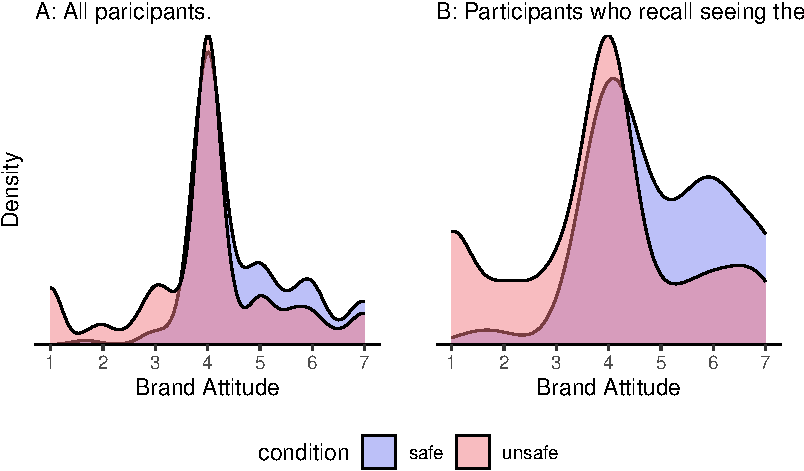
\includegraphics{project_dice_files/figure-pdf/fig-main-effects-1.pdf}

}

\caption{\label{fig-main-effects}Effect of Misplaced Ad on Brand
Evaluations}

\end{figure}

This effect becomes even stronger if we only consider those participants
who recall seeing the ad: The unsafe feed (\(M_u = 3.81\)) resulted in
significantly less favorable brand evaluations than the more general
feed (\(M_s = 5.02\), \(F(1, 296) = 21.71\), \(p = 0.000\),
\(\text{Cohen's d} = 0.8\)).
\texttt{{[}Check\ wheher\ there\ are\ differences\ between\ recall\ measures\ (aided\ vs.\ unaided)\ to\ better\ understand\ implicit\ memory\ effects.{]}}

We illustrate both effects in panel A and B of Figure
Figure~\ref{fig-main-effects}, respectively. Comparing both panels, one
can see that the density around the center diminishes once one considers
only those participants who remember (aided recall) that they have been
exposed to an ad.

\textbf{Recall.}
\texttt{{[}If\ we\ use\ this\ study\ to\ demonstrate\ the\ context-contribution,\ we\ don\textquotesingle{}t\ need\ dwell\ time\ analyses\ here.{]}}
A logit regression provides correlational evidence which indicates that
an additional second in the viewport increases the odds of recall by
about 3\% holding other factors constant (\(p = 0.01\)). Controlling for
the experimental condition this value changes only slightly\footnote{An
  additional second in the viewport increases the odds of recall by
  about 1.05\% (\(p = 0.02\))}. The interaction's large standard error
in Model 2 presented in Table~\ref{tbl-recall-regressions} indicates
that this correlation is robust across conditions.

\hypertarget{tbl-recall-regressions}{}
\begin{longtable}[]{@{}
  >{\raggedright\arraybackslash}p{(\columnwidth - 16\tabcolsep) * \real{0.2759}}
  >{\centering\arraybackslash}p{(\columnwidth - 16\tabcolsep) * \real{0.0690}}
  >{\centering\arraybackslash}p{(\columnwidth - 16\tabcolsep) * \real{0.1121}}
  >{\centering\arraybackslash}p{(\columnwidth - 16\tabcolsep) * \real{0.0690}}
  >{\centering\arraybackslash}p{(\columnwidth - 16\tabcolsep) * \real{0.1121}}
  >{\centering\arraybackslash}p{(\columnwidth - 16\tabcolsep) * \real{0.0690}}
  >{\centering\arraybackslash}p{(\columnwidth - 16\tabcolsep) * \real{0.1121}}
  >{\centering\arraybackslash}p{(\columnwidth - 16\tabcolsep) * \real{0.0690}}
  >{\centering\arraybackslash}p{(\columnwidth - 16\tabcolsep) * \real{0.1121}}@{}}
\caption{\label{tbl-recall-regressions}Logit Results}\tabularnewline
\toprule\noalign{}
\begin{minipage}[b]{\linewidth}\raggedright
\textbf{Characteristic}
\end{minipage} & \begin{minipage}[b]{\linewidth}\centering
\textbf{OR}
\end{minipage} & \begin{minipage}[b]{\linewidth}\centering
\textbf{p-value}
\end{minipage} & \begin{minipage}[b]{\linewidth}\centering
\textbf{OR}
\end{minipage} & \begin{minipage}[b]{\linewidth}\centering
\textbf{p-value}
\end{minipage} & \begin{minipage}[b]{\linewidth}\centering
\textbf{OR}
\end{minipage} & \begin{minipage}[b]{\linewidth}\centering
\textbf{p-value}
\end{minipage} & \begin{minipage}[b]{\linewidth}\centering
\textbf{OR}
\end{minipage} & \begin{minipage}[b]{\linewidth}\centering
\textbf{p-value}
\end{minipage} \\
\midrule\noalign{}
\endfirsthead
\toprule\noalign{}
\begin{minipage}[b]{\linewidth}\raggedright
\textbf{Characteristic}
\end{minipage} & \begin{minipage}[b]{\linewidth}\centering
\textbf{OR}
\end{minipage} & \begin{minipage}[b]{\linewidth}\centering
\textbf{p-value}
\end{minipage} & \begin{minipage}[b]{\linewidth}\centering
\textbf{OR}
\end{minipage} & \begin{minipage}[b]{\linewidth}\centering
\textbf{p-value}
\end{minipage} & \begin{minipage}[b]{\linewidth}\centering
\textbf{OR}
\end{minipage} & \begin{minipage}[b]{\linewidth}\centering
\textbf{p-value}
\end{minipage} & \begin{minipage}[b]{\linewidth}\centering
\textbf{OR}
\end{minipage} & \begin{minipage}[b]{\linewidth}\centering
\textbf{p-value}
\end{minipage} \\
\midrule\noalign{}
\endhead
\bottomrule\noalign{}
\endlastfoot
seconds\_in\_viewport & 1.03 & 0.008 & 1.05 & 0.025 & & & & \\
condition & & & 1.72 & 0.13 & & & 1.84 & 0.12 \\
seconds\_in\_viewport * condition & & & & & & & & \\
seconds\_in\_viewport * unsafe & & & 0.97 & 0.2 & & & & \\
relative\_dwell\_time & & & & & 24.1 & 0.091 & 268 & 0.057 \\
relative\_dwell\_time * condition & & & & & & & & \\
relative\_dwell\_time * unsafe & & & & & & & 0.01 & 0.3 \\
\end{longtable}

\texttt{{[}Because\ we\ analyze\ dwell\ time\ in\ the\ next\ study\ in\ more\ detail,\ we\ should\ use\ it\ here\ to\ exclude\ participants\ who\ have\ not\ paid\ attention\ to\ the\ ad:\ either\ exclude\ them\ or\ control\ for\ dwell\ time\ on\ focal\ post.{]}}

\hypertarget{dwell-time-case}{%
\subsection{Dwell Time Case}\label{dwell-time-case}}

Lorem ipsum.

\hypertarget{future-opportunities-from-using-dice-in-marketing-research}{%
\section{Future Opportunities from using DICE in Marketing
Research}\label{future-opportunities-from-using-dice-in-marketing-research}}

The current paper proposes a novel paradigm, DICE, to conduct research
that has the capacity to keep the advantages of classic vignette studies
(e.g., high experimental control to maximize internal validity) and
advantages of observational and online platform studies (e.g., high
realism to maximize ecological validity) while eliminating their main
disadvantages and methodological issues discussed in prior work (see
Table 1). DICE also enables researchers to measure content engagement
with maximal resolution at the individual level, which was not possible
in any of the currently used social media research designs (e.g.,
millisecond dwell time response measures at the feed level or sequential
content browsing trajectories during a session). These features allow
researchers to pursue entirely new lines of inquiry in future social
media research. In what follows, we discuss the methodological
contributions and offer directions for future work and how DICE could be
utilized to make better-informed decisions for key players in the social
media ecosystem (e.g., brands, influencers, platform providers,
agencies, and public policy).

\hypertarget{methodological-implications}{%
\subsection{Methodological
Implications}\label{methodological-implications}}

The methodological contributions of DICE directly address several
challenges in the research designs employed in prior social media
research. First, DICE ensures stable group assignment by eliminating
divergent delivery and issues with potentially multiple exposures in
online platform studies. DICE, therefore, directly addresses the
limitations of ``black box'' engagement algorithms on all major social
media platforms and the lack of control for researchers to study truly
causal effects on these platforms.

Second, and as a consequence, DICE offers high ecological value that
closely mimics the environments in online platform studies or
observational studies but with the additional advantage of offering feed
composition controls in which researchers can directly specify the mode
and sequence of how content should be delivered across conditions. This
researcher-controlled delivery overcomes the methodological drawbacks of
typical observational studies (e.g., endogeneity) and online platform
studies (e.g., divergent delivery), while offering a similar level of
control as vignettes.

Third, DICE offers the ability to measure content engagement with high
resolution at the individual level, which was not possible before
without extensive monetary and time investments. DICE allows researchers
to track millisecond dwell time content engagement and sequential
content trajectories at the individual level. Thus, researchers can
directly measure the relative content engagement, a proxy for consumer
attention, at a highly atomized level for every single post or item in a
feed and the sequence of content consumption (e.g., whether users read a
post, then scroll down and up again). The metrics produced from this
tracking data in DICE offer a new lens to study attention-related
mechanisms in future social media research (see our future research
directions section).

Fourth, DICE directly integrates crowdsourcing platforms for participant
recruitment, such as Prolific or Amazon Mechanical Turk, to track
participant identifiers across the entire duration of a study and also
integrates with survey management platforms, such as Qualtrics, to
follow up with post-survey measurements after exposure to different
treatment conditions. Thus, our paradigm combines behavioral tracking
data and traditional survey instruments within a single study. While the
tracking data is theoretically available in online platform studies, it
is typically inaccessible for researchers as it is used to ``optimize''
engagement metrics (and, in turn, jeopardizes the possibility of drawing
causal inferences). Finally, we designed DICE as an easy-to-use,
low-cost, open-source environment to promote replicability and
transparency for all researchers. Our aim is to offer a paradigm and
platform to conduct robust, high-quality social media research studies,
that directly address the lack of transparency, replicability, and
customization on major social media platforms.

\hypertarget{future-research-directions}{%
\subsection{Future Research
Directions}\label{future-research-directions}}

In what follows, we outline future directions for key actors and
stakeholders in the social media ecosystem (i.e., marketing scholars,
brands, influencers, agencies, and public policy) on how DICE offers the
possibility to explore either new phenomena or to utilize the
methodological advantages to deepen our understanding of previously
studied phenomena. We offer a summary of selected and exemplary
questions in Table 2.

\hypertarget{concluding-thoughts}{%
\section{Concluding Thoughts}\label{concluding-thoughts}}

In this paper, we have introduced DICE, a novel experimental paradigm,
along with a user-friendly, open-source research app that resolves key
methodological issues in social media research while enhancing
ecological value and causal inference. DICE represents a synthesis of
the advantages of high experimental control (and therefore internal
validity) found in scenario-based vignette studies with the advantages
of high realism (and therefore ecological validity) of observational and
platform studies. Our DICE paradigm, along with the behavioral tracking
possibilities to assess attention and scrolling trajectories with high
resolution at the individual level, offers new avenues for rigorous,
realistic, and ultimately relevant marketing research for a wide range
of stakeholders within the social media ecosystem. Given DICE's modular
nature, it is also possible to further adapt the environment to just any
other platform featuring scrollable content streams.
\texttt{{[}Show\ how\ and\ under\ which\ conditions\ in\ Appendix.{]}}
For example, professional networks like LinkedIn, online review
platforms like Yelp or e-commerce sites like Amazon could be modeled to
test messaging effects on engagement, recruitment, product search, and
purchasing behavior with high resolution. This adaptability of DICE
underscores its capacity for broad application across various online
environments, each with its idiosyncratic user engagement dynamics and
commercial and theoretical implications (see also Swaminathan et al.
2023). In summary, DICE presents a novel research paradigm to examine
important marketing questions in social media and other digital
contexts.

\hypertarget{the-price-of-civility-economic-and-social-returns-on-investment-in-toxicity-moderation}{%
\chapter{The Price of Civility: Economic and Social Returns on
Investment in Toxicity
Moderation}\label{the-price-of-civility-economic-and-social-returns-on-investment-in-toxicity-moderation}}

\emph{Meta} estimates its users create approximately
\href{https://web.archive.org/web/20240531061745/https://www.facebook.com/business/news/stories-can-do-it}{one
billion} stories---ephemeral posts---daily. Stylistically, each
additional post augments the appeal of platforms like Meta, TikTok, and
X because it contributes potentially novel and diverse content to a
massive content pool. To tame the scale of these content pools and to
ensure that its size indeed augments a platform's appeal, one of the
platforms' most critical functions is to distribute the most relevant
content per user.\footnote{In addition to facilitating the content
  production and consumption, the core of a platform's business is to
  distribute the content to its consumers. Due to the unprecedented
  scale of content production, social media platforms cannot expose all
  of its users to all the available content. Instead, they curate
  personalized subsets of content. In contrast to traditional media
  outlets, where editors select content for a broad audience,
  recommender systems on these platforms generate tailored lists of
  content for individual users.} Well-designed content recommendations
tend to positively affect the duration of user engagement (Aridor et al.
2024), which is crucial for platforms because advertisers are interested
in capturing users' attention and pay these platforms to gain a share of
it. This is so significant that digital advertising, a substantial
portion of which is placed on social media, now accounts for most of
global advertising expenditures (Deisenroth et al. 2024).

Formally, a social platform chooses a targeting rule that picks, for
each user \(i\), a personalized subset \(\mathbf{x}_i\) from the total
pool of posts to show the user. A post is characterized by a vector of
characteristics, \(x \in \mathbb{R}^K\) which can include, for example,
toxicity or sentiment expressed. Platforms choose the posts that
maximize the revenue-weighted time spent \((t_i(\mathbf{x}_i))\) on the
platform. \(\alpha(\mathbf{x}_i)\) represents the monetary gains the
platform gets per unit of time spent from showing \(\mathbf{x}_i\) to
\(i\) (Aridor et al. 2024, 3). In addition, the platform faces costs
\(c(\mathbf{N}, \mathbf{M})\) that increases in the total numbers of
users \(\mathbf{N}\) and posts \(\mathbf{M}\). These may include the
technical infrastructure as well as labor costs.

\[
\max_{\{\mathbf{x}_i\} \subseteq U; \mathbf{x}_j^p} \left( \sum_i \alpha(\mathbf{x}_i) t_i(\mathbf{x}_i) - c(\mathbf{N}, \mathbf{M}) \right)
\]

One specific driver of costs is content moderation: Despite selecting
potentially relevant content per user, platforms also have to filter
content that should \emph{not} be displayed to any user. Because
platforms cannot control the content production directly, they typically
set rules that define which type of content shall (not) be displayed.
However, actively moderating the content production by enforcing these
rules and sanctioning violations is costly because platforms need to
design algorithms that flag potentially unwanted content and employ
human moderators who evaluate the flagged posts. These are considered
\emph{direct} costs and represented by \(c(\mathbf{N}, \mathbf{M})\).

In addition, there may be \emph{indirect} costs because field
experimental evidence suggests that the removal of harmful
content\footnote{This includes hate speech and misinformation, for
  instance, and is considered harmful as the literature works with the
  assumption that such content imposes negative externalities on groups
  of the population (Beknazar-Yuzbashev et al. 2022, 8)} reduces content
consumption. Hence, and perhaps counterintuitively, \(t(\cdot)\)
decreases in \(\mathbf{x}_i\)'s civility. However, anecdotal evidence
suggests that advertisers react to harmful content by withdrawing their
campaign budget for platforms that promote such content. In November
2023, CNN reported that at least a dozen major brands, such as IBM or
Disney, halted their ad spending over concerns about antisemitism and
hate speech on X. Such \emph{brand safety} measures indicate that
\(\alpha(\cdot)\) may increase in \(\mathbf{x}_i\)'s civility. Moreover,
Ahmad et al. (2024) find that most brand managers prefer their
advertisements not to be displayed on websites that distribute
misinformation and lack civility.

Focusing on one specific form of uncivil content, it is not clear how
the product of \(\alpha(\cdot)t(\cdot)\) is affected by toxicity. This
study aims to find out.

\hypertarget{the-sound-of-certainty-assessing-paralinguistic-indicators-of-decision-confidence}{%
\chapter{The Sound of Certainty: Assessing Paralinguistic Indicators of
Decision
Confidence}\label{the-sound-of-certainty-assessing-paralinguistic-indicators-of-decision-confidence}}

Co-authored with Max Gaerth (Wharton) and Christian Hildebrand
(University of St.~Gallen), we have completed a pre-test as well as the
first study. We are currently refining two additional studies, for which
the experimental designs and software have already been developed, while
the fourth study has not yet commenced. We plan to submit our findings
to the Journal of Marketing Research, which is renowned for welcoming
methodological contributions and for its high visibility within our
research community.

\hypertarget{introduction-2}{%
\section{Introduction}\label{introduction-2}}

The average adult makes about 35,000 remotely conscious decisions each
day. In fact, we make 226.7 decisions each day on just food alone
\texttt{(Hoomans\ 2015)}. Many of which can be thought of as trade-offs
(see, e.g. Shaddy, Fishbach, and Simonson 2021 for a recent review).
Think of a restaurant customer who chooses a protein for her ramen soup.
She can choose between pork or chicken, for instance, and intuitively
decides whether and how much to satisfy one consideration at the expense
of another.

To understand how consumers resolve such trade-offs, prior research has
established that the strength of consumer preferences, defined as the
confidence with which consumers hold their preferences and the stability
of their preferences over time, plays a pivotal role (e.g., Amir and
Levav 2008; Yoon and Simonson 2008). To measure preference strength,
researchers have traditionally relied on retrospective methods, such as
questionnaire measures and conjoint analayses. These \emph{direct}
approaches rely on two strong assumptions: people are able to introspect
their psychological states, and they are willing to report correctly the
results of their introspection (Fischer et al. 2023, 2). To relax these
assumptions, researchers have begun to append direct measures with
response times. Response times are a promising \emph{indirect} measure,
that can be elicited unobtrusively and that reveals more information
(than discrete choices stated in retrospective methods) because it is
continuous. An extensive body of literature established that longer
response times are associated to lower preference strength (see, e.g.,
Luce 1991; Bergert and Nosofsky 2007; Bhatia and Mullett 2018). However,
response times can be noisy as they also capture many constructs
unrelated to decisions (Konovalov and Krajbich 2019).

This research also focuses on \emph{how} decisions are transmitted but
considers vocal instead of manual communication. Vocal communication
involves more than just the words that echo a decision (Mehrabian 1971;
Gorodnichenko, Pham, and Talavera 2023) and comprises non-verbal
elements such as tone, pitch, or pace (see, e.g., Zierau et al. 2023;
Melzner, Bonezzi, and Meyvis 2023). These so-called
\emph{paralinguistics} can not only be measured continuously but also
less controllable and more immediate. Contemplation, for instance, is
associated with slower speech with longer pauses (Dasgupta 2017), anger
is often associated with louder speech, and fear with greater pitch
variability (Juslin and Laukka 2003; Clark 2005). Hence, paralinguistics
offer a unique and unintended lens to reveal one's inner thoughts and
feelings that cannot be retrieved from text transcript.

Consider the ramen example again. Suppose we are attempting to determine
which of two people, Peter or Bob, is more confident in his choice and
suppose that both order pork with the exact same wording. With just this
information there is no way to distinguish between them. Now suppose
Peter orders loudly and clearly, whereas Bob may speak more quietly,
raising the intonation at the end of the statement as if he was asking a
question. Who has a stronger preference for one protein over the other?
Since Peter communicated his choice more confidently than Bob, it is
likely that he found it more delicious. In other words, Peter's relative
preference for pork was likely stronger than Bob's; he was farther from
indifference (i.e., the point at which she is equally likely to choose
either option). Of course, if Peter and Bob differ on relevant
characteristics such as age or culture, we might be misled about their
preferences. It is thus an empirical question whether our example is
actually feasible or speculation. This is a key question that we tackle
in this paper.

The answer to this question has practical implications because voice
analytics (i.e., the computational extraction of paralinguistics) is
increasingly available to marketers as voice data is becoming
ubiquitous. Due to the rise of voice-enabled technology and chat
interfaces, consumers who used to search for information, make bank
transactions, and choose products using only their keyboard or mouse,
can now perform almost any computer-based task using voice commands. In
2022, it was estimated that 62\% of all Americans aged 18 or older used
some type of voice-enabled technology (e.g., smart devices), and of
these, 57\% indicated using voice technology daily (NPR and Edison
Research 2022). Notably, one can easily imagine the adoption to further
increase as major companies, such as Apple, released the first version
of \emph{Apple Intelligence}, its suite of artificial intelligence
features that will improve their voice assistant Siri based on OpenAI's
ChatGPT (Malik 2024).

Building on the findings on preference strength, we hypothesize that
certain vocal features will change as a function of consumers' strength
of preferences. To test this hypothesis, we utilize the technological
advances mentioned above, chat interfaces and large language models, in
a series of four studies that we outline below.

\hypertarget{study-1}{%
\section{Study 1}\label{study-1}}

The goal of Study 1 was to examine (a) whether preference strength on a
given trial predicted how participants vocalized their choice (i.e.,
vocal features) and (b) whether vocal features could be used to predict
preference strength.

\textbf{Participants:} 242 Prolific panelists (\(M_{age} =\) 39.96,
\(SD_{age} =\) 13.14; 36\% female) completed the study. We based our
sample size on past work using within−subjects designs and a
mouse−tracking task (cite). The study employed a 2 (conflict: low
vs.~high) × 2 (gender model: male vs.~female) × 2 (replicates)
within-subjects design.

\textbf{Procedure and stimuli:} Participants completed eight choice
trials between two models. To induce differences in participants'
preference strength across all eight trials, we manipulated the
decisional conflict associated with these choice trials. We pre-tested a
variety of model headshots to identify pairs with high decisional
conflict (where both models were equally attractive) and low decisional
conflict (where one model was perceived as being more attractive on
average). More information on the pre-test as well as the specific
stimuli can be found in Section~\ref{sec-sound-pre-test} and
Section~\ref{sec-sound-stimuli}, respectively. Importantly, the
presentation order of the models as well as pairs was randomized within
participants. For each choice trial, participants were asked to say out
loud which of the two models they find more attractive. After each
choice, participants indicated the strength of their preference on a
101−point slider scale (i.e., 0 = Strong preference for Model X, 1 =
strong preference for Model Y) on a separate page.

Before the start of the study, participants completed two trial rounds
to familiarize themselves with the recording interface and test (or
adjust) their settings to ensure a high audio quality. Subsequently,
participants were led through the choice task described above. Lastly,
participants indicated their age, gender, and environmental factors that
could affect the quality of their recordings or trigger
self-presentational concerns. Accordingly, they indicated whether they
were alone or in a public space and whether they disguised their voice.

\textbf{Results:} These results suggest that vocal features can be a
sensitive metric for strength of preferences within a given decision and
that the variance is distinct from established implicit measures, such
as response time.

\textbf{Discussion:}

\hypertarget{study-2}{%
\section{Study 2}\label{study-2}}

Participants will be randomly assigned to a 10-trial repeated measures
design. They will indicate their preferred product version between two
options (e.g., Diet Coke vs.~Coke Zero) using a voice interface designed
with oTree (Chen, Schonger, and Wickens 2016) and OpenAI's \emph{Whisper
API}.\footnote{Our oTree app extends functions provided in McKenna
  (2024)}

Subsequently, participants will engage in a titration task for each of
the 10 trials, where the price of the preferred product version will be
increased incrementally (from 5\% to 40\% in 5\% steps). For each price
premium, participants will indicate whether they would choose to buy the
preferred product version, or the less preferred product version.

This process will allow us to determine our outcome variable: the
maximum acceptable price premium (MAPP) a participant would pay before
switching to the less preferred product. Specifically, we will examine
the relationship between preference strength, as measured by
paralinguistic features, and MAPP. We hypothesize that consumers'
preference strength for one product over the other (which we approximate
using the paralinguistic features) will significantly predict MAPP.

\hypertarget{study-3}{%
\section{Study 3}\label{study-3}}

In a first study, we ask whether we can learn how hard a decision is not
by listening to \emph{what} consumers say but \emph{how} they say it.

\textbf{Experimental Paradigm:} We employ a Multiple Price List design
(see, e.g., Andersen et al. 2006) and expose study participants to a
series of ten decisions that differ with respect to their decision
difficulty. More precisely, participants choose between two artificial
products that differ only in their product ratings. Whereas the
lower-rated product has a fixed price in each decision, the price of the
higher-rated product varies between decisions. Table~\ref{tbl-stimuli}
summarizes these decisions.

\hypertarget{tbl-stimuli}{}
\begin{longtable}[]{@{}rrrrr@{}}
\caption{\label{tbl-stimuli}Manipulation of Dicision
Difficulty}\tabularnewline
\toprule\noalign{}
Decision & Quality A & Quality B & Price A & Price B \\
\midrule\noalign{}
\endfirsthead
\toprule\noalign{}
Decision & Quality A & Quality B & Price A & Price B \\
\midrule\noalign{}
\endhead
\bottomrule\noalign{}
\endlastfoot
1 & 3.8 & 4.2 & 200 & 200 \\
2 & 3.8 & 4.2 & 200 & 204 \\
3 & 3.8 & 4.2 & 200 & 209 \\
4 & 3.8 & 4.2 & 200 & 213 \\
5 & 3.8 & 4.2 & 200 & 218 \\
6 & 3.8 & 4.2 & 200 & 226 \\
7 & 3.8 & 4.2 & 200 & 232 \\
8 & 3.8 & 4.2 & 200 & 240 \\
9 & 3.8 & 4.2 & 200 & 246 \\
10 & 3.8 & 4.2 & 200 & 254 \\
\end{longtable}

Because both products share the same price in the first decision but
differ with respect to their quality, product B weakly dominates product
A. With these information being salient, consumers should choose product
B and, importantly, they should be confident in choosing between the
two.

As the price of product B increases over the course of the following
decisions, the consumers face a trade-off between price and quality.
Notably, this trade-off becomes more difficult as the price increases up
to the point where product B becomes too expensive. From that so-called
switching point on, the trade-off difficulty should decrease again.
\texttt{{[}How\ does\ decision\ difficulty\ relate\ to\ decision\ confidence?{]}}

As a consequence, we expect the confidence with which consumers make
these decisions to exhibit a U-shaped pattern that we illustrate for 100
simulated participants in Figure~\ref{fig-sawtooth}.

\begin{figure}

{\centering 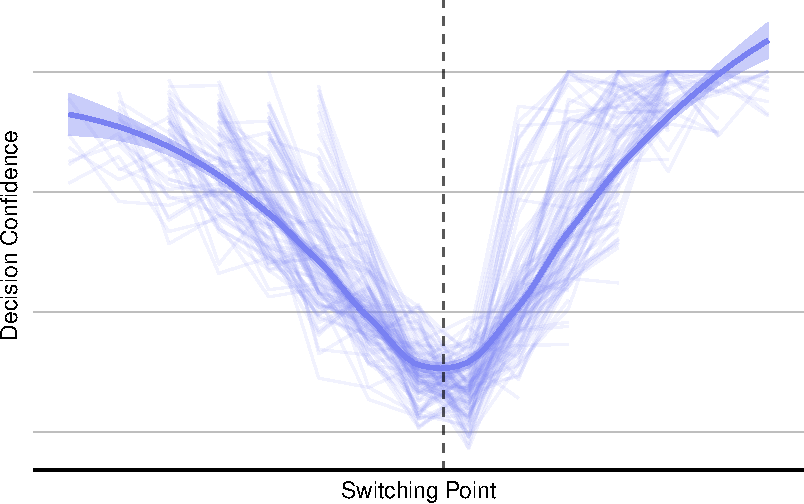
\includegraphics{project_sounds_files/figure-pdf/fig-sawtooth-1.pdf}

}

\caption{\label{fig-sawtooth}Expected U-Shape Pattern in Choice
Confidence}

\end{figure}

Crucially, participants communicate their decisions verbally as they
make their respective choices. This enables us to not only measure
\emph{what} they say (to localize their switching points) but also to
measure \emph{how} they say it during a time closely aligned with their
decision-making process.

To sum up, we build on an established paradigm that yields clear and
intuitive predictions and modify it to record rich audio information
which we can decode, transcribe and analyze to get a glimpse into the
underlying psychological states that drive decision-making.

\textbf{Validation:} We tested this prediction in pre-test that was
conducted online and where participants entered their preference
strength manually using a slider. We recruited participants via Prolific
and classified 68 participants as rational because they were only
switching once. The resulting pattern, illustrated in
Figure~\ref{fig-reality}, matches the prediction.

\begin{figure}

{\centering 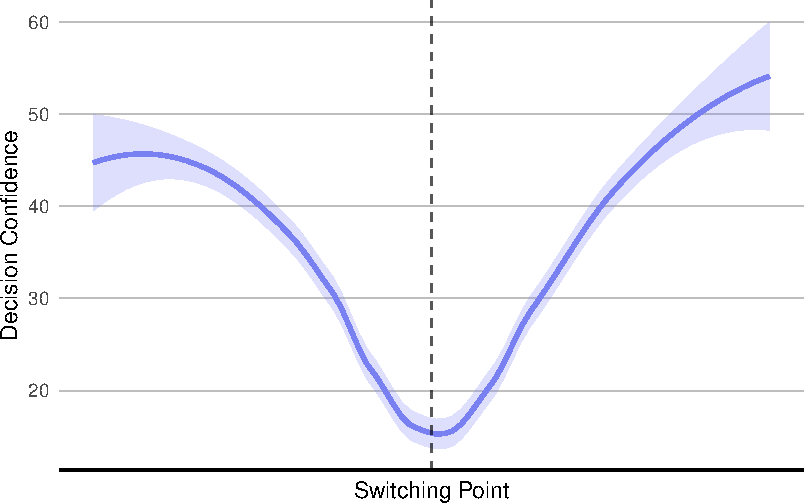
\includegraphics{project_sounds_files/figure-pdf/fig-reality-1.pdf}

}

\caption{\label{fig-reality}Fitted Pattern in Self-Reported Choice
Confidence}

\end{figure}

\textbf{Identification:} To learn whether we could describe the latent
consumer confidence, we build on the experimental paradigm and the
expected confidence pattern described above and illustrated in
Figure~\ref{fig-sawtooth} and Figure~\ref{fig-reality}. In addition to
the pre-test reported above, we will run another study where we will
change the modality and ask participants to voice their decision. This
will yield ten voice recordings per participant which we will use to
extract the same vocal features we extracted in the previous studies.
Building on the findings of Study 1 and Study 2, we can put the features
with the highest predicted power to yet another test and (correlate and)
plot them against the U-shape derived above.

\hypertarget{study-4}{%
\section{Study 4}\label{study-4}}

To promote the consumption, adoption, and ongoing usage of our research
findings, we plan to develop a customized deep learning model for
detecting preference strength in speech. To this end, we hire 24 North
American voice actors and actresses who will speak statements in with
varying degrees of certainty (uncertain, neutral, certain) and recruit
Prolific participants for validation. Using these data, we will follow
Gorodnichenko, Pham, and Talavera (2023) and use Librosa, a Python
package, to extract vocal features. More specifically, we will extract
128 mel spectrogram frequencies which allows us to determine the level
of loudness of a particular frequency at a particular time for each
recording. In addition, a chromagram with 12 chroma coefficients will be
extracted. The chromagram reflects the distribution of energy along 12
chroma bands (i.e., C, C\#, D, D\#, E, F, F\#, G, G\#, A, A\#, and B)
over time and, hence, can capture melodic and harmonic characteristics
of audio. Moreover, we will extract 40 mel-frequency cepstral
coefficients (MFCCs), which are discrete cosine transformations of the
mel frequency spectrogram (as Gorodnichenko, Pham, and Talavera (2023)
found it to improve their model).

After extracting the vocal features from each recording our data, we
have a labeled dataset that split into training and testing data. We use
the training subset to build and fine-tune a neural network using an
established deep learning framework such as \emph{Keras}.\footnote{Alternatively,
  we can also try to fine-tune an existing model such as Facebook's
  \href{https://huggingface.co/facebook/wav2vec2-base}{Wav2Vec}, which
  is described
  \href{https://huggingface.co/docs/transformers/en/tasks/audio_classification}{here}.}
The testing data will then be used to evaluate the model's performance
using the following accuracy score:

\[
\text{Accuracy}(y, \hat{y}) = \frac{1}{n} \sum_{i=1}^n \mathbf{1}\{\hat{y}_i = y_i\}
\]

where \(y\) and \(\hat{y}\) are the true and the predicted levels of
certainty, respectively, and \(n\) is the number of audio files in the
testing dataset.

\part{OUTLOOK}

\hypertarget{work-plan}{%
\chapter{Work Plan}\label{work-plan}}

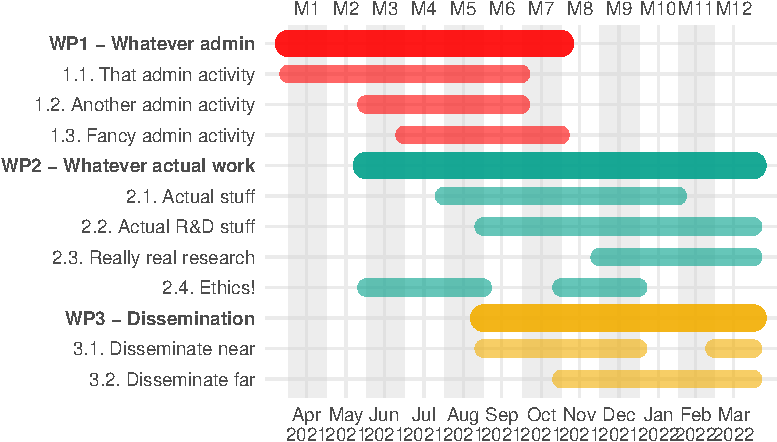
\includegraphics{timeline_files/figure-pdf/unnamed-chunk-1-1.pdf}

\hypertarget{outcomes-and-impact}{%
\chapter{Outcomes and Impact}\label{outcomes-and-impact}}

Mention expected outcomes here.

\bookmarksetup{startatroot}

\hypertarget{references}{%
\chapter*{References}\label{references}}
\addcontentsline{toc}{chapter}{References}

\markboth{References}{References}

\begingroup
\raggedright

\hypertarget{refs}{}
\begin{CSLReferences}{1}{0}
\leavevmode\vadjust pre{\hypertarget{ref-AhmadEtAl_2024}{}}%
Ahmad, Wajeeha, Ananya Sen, Charles Eesley, and Erik Brynjolfsson. 2024.
{``Companies Inadvertently Fund Online Misinformation Despite Consumer
Backlash.''} \emph{Nature} 630: 123--31.
\url{https://doi.org/10.1038/s41586-024-07404-1}.

\leavevmode\vadjust pre{\hypertarget{ref-AllcottGentzkowSong_2022}{}}%
Allcott, Hunt, Matthew Gentzkow, and Lena Song. 2022. {``Digital
Addiction.''} \emph{American Economic Review} 112 (7): 2424--63.
\url{https://doi.org/10.1257/aer.20210867}.

\leavevmode\vadjust pre{\hypertarget{ref-AmirLevav_2008}{}}%
Amir, On, and Jonathan Levav. 2008. {``Choice Construction Versus
Preference Construction: The Instability of Preferences Learned in
Context.''} \emph{Journal of Marketing Research} 45 (2): 145--58.
\url{https://doi.org/10.1509/jmkr.45.2.145}.

\leavevmode\vadjust pre{\hypertarget{ref-AndersenEtAl_2006}{}}%
Andersen, Steffen, Glenn W. Harrison, Morten Igel Lau, and E. Elisabet
Rutström. 2006. {``Elicitation Using Multiple Price List Formats.''}
\emph{Experimental Economics} 9 (4): 383--405.
\url{https://doi.org/10.1007/s10683-006-7055-6}.

\leavevmode\vadjust pre{\hypertarget{ref-AndersonWood_2021}{}}%
Anderson, Ian A., and Wendy Wood. 2021. {``Habits and the Electronic
Herd: The Psychology Behind Social Media's Successes and Failures.''}
Journal Article. \emph{Consumer Psychology Review} 4 (1): 83--99.
\url{https://doi.org/10.1002/arcp.1063}.

\leavevmode\vadjust pre{\hypertarget{ref-AngristPischke_2009}{}}%
Angrist, Joshua D., and Jörn-Steffen Pischke. 2009. \emph{Mostly
Harmless Econometrics: An Empiricist's Companion}. Princeton university
press.

\leavevmode\vadjust pre{\hypertarget{ref-AppelEtAl_2020}{}}%
Appel, Gil, Lauren Grewal, Rhonda Hadi, and Andrew T. Stephen. 2020.
{``The Future of Social Media in Marketing.''} Journal Article.
\emph{Journal of the Academy of Marketing Science} 48 (1): 79--95.
\url{https://doi.org/10.1007/s11747-019-00695-1}.

\leavevmode\vadjust pre{\hypertarget{ref-AppelMarkerGnambs_2020}{}}%
Appel, Markus, Caroline Marker, and Timo Gnambs. 2020. {``Are Social
Media Ruining Our Lives? A Review of Meta-Analytic Evidence.''} Journal
Article. \emph{Review of General Psychology} 24 (1): 60--74.
\url{https://doi.org/10.1177/1089268019880891}.

\leavevmode\vadjust pre{\hypertarget{ref-Aridor_2024}{}}%
Aridor, Guy. 2024. {``Measuring Substitution Patterns in the Attention
Economy: An Experimental Approach.''} \emph{SSRN Electronic Journal}.
\url{https://doi.org/10.2139/ssrn.4069567}.

\leavevmode\vadjust pre{\hypertarget{ref-AridorEtAl_2024}{}}%
Aridor, Guy, Rafael Jiménez-Durán, Ro'ee Levy, and Lena Song. 2024.
{``The Economics of Social Media.''} \emph{Journal of Economic
Literature}. \url{https://doi.org/10.2139/ssrn.4723727}.

\leavevmode\vadjust pre{\hypertarget{ref-BaumesiterVohsFunder_2007}{}}%
Baumeister, Roy F., Kathleen D. Vohs, and David C. Funder. 2007.
{``Psychology as the Science of Self-Reports and Finger Movements:
Whatever Happened to Actual Behavior?''} \emph{Perspectives on
Psychological Science} 2 (4): 396--403.
\url{https://doi.org/10.1111/j.1745-6916.2007.00051.x}.

\leavevmode\vadjust pre{\hypertarget{ref-BeknazarYuzbashevEtAl_2022}{}}%
Beknazar-Yuzbashev, George, Rafael Jiménez Durán, Jesse McCrosky, and
Mateusz Stalinski. 2022. {``Toxic Content and User Engagement on Social
Media: Evidence from a Field Experiment.''} SSRN Working Paper. SSRN.
\url{https://doi.org/10.2139/ssrn.4307346}.

\leavevmode\vadjust pre{\hypertarget{ref-BellmanEtAl_2018}{}}%
Bellman, Steven, Ziad H. S. Abdelmoety, Jamie Murphy, Shruthi
Arismendez, and Duane Varan. 2018. {``Brand Safety: The Effects of
Controversial Video Content on Pre-Roll Advertising.''} \emph{Heliyon} 4
(12): e01041. \url{https://doi.org/10.1016/j.heliyon.2018.e01041}.

\leavevmode\vadjust pre{\hypertarget{ref-BergerMilkman_2016}{}}%
Berger, Jonah, and Katherine L. Milkman. 2012. {``What Makes Online
Content Viral?''} \emph{Journal of Marketing Research} 49 (2): 192--205.
\url{https://doi.org/10.1509/jmr.10.0353}.

\leavevmode\vadjust pre{\hypertarget{ref-BergerMoeSchweidel_2023}{}}%
Berger, Jonah, Wendy W. Moe, and David A. Schweidel. 2023. {``What Holds
Attention? Linguistic Drivers of Engagement.''} \emph{Journal of
Marketing} 87 (5): 793--809.
\url{https://doi.org/10.1177/00222429231152880}.

\leavevmode\vadjust pre{\hypertarget{ref-BergertNosofsky_2007}{}}%
Bergert, F. B., and R. M. Nosofsky. 2007. {``A Response-Time Approach to
Comparing Generalized Rational and Take-the-Best Models of Decision
Making.''} \emph{Journal of Experimental Psychology: Learning, Memory,
and Cognition} 33 (1): 107--29.
\url{https://doi.org/10.1037/0278-7393.33.1.107}.

\leavevmode\vadjust pre{\hypertarget{ref-BhatiaMullet_2018}{}}%
Bhatia, S., and T. L. Mullett. 2018. {``Similarity and Decision Time in
Preferential Choice.''} \emph{Quarterly Journal of Experimental
Psychology} 71 (6): 1276--80.
\url{https://doi.org/10.1177/1747021818763054}.

\leavevmode\vadjust pre{\hypertarget{ref-BoegershausenEtAl_2022}{}}%
Boegershausen, Johannes, Hannes Datta, Abhishek Borah, and Andrew T.
Stephen. 2022. {``Fields of Gold: Scraping Web Data for Marketing
Insights.''} \emph{Journal of Marketing} 86 (5): 1--20.
\url{https://doi.org/10.1177/00222429221100750}.

\leavevmode\vadjust pre{\hypertarget{ref-BraunEtAl_2024}{}}%
Braun, Michael, Bart de Langhe, Stefano Puntoni, and Eric M Schwartz.
2024. {``Leveraging Digital Advertising Platforms for Consumer
Research.''} \emph{Journal of Consumer Research} 51 (1): 119--28.
\url{https://doi.org/10.1093/jcr/ucad058}.

\leavevmode\vadjust pre{\hypertarget{ref-BraunSchwartz_2023}{}}%
Braun, Michael, and Eric M Schwartz. 2023. {``Where AB Testing Goes
Wrong: What Online Experiments Cannot (and Can) Tell You about How
Customers Respond to Advertising.''} \emph{SMU Cox School of Business
Research Paper}, no. 21-10. \url{https://doi.org/10.2139/ssrn.3896024}.

\leavevmode\vadjust pre{\hypertarget{ref-oTree}{}}%
Chen, Daniel L., Martin Schonger, and Chris Wickens. 2016. {``oTree---an
Open-Source Platform for Laboratory, Online, and Field Experiments.''}
\emph{Journal of Behavioral and Experimental Finance} 9: 88--97.
\url{https://doi.org/doi.org/10.1016/j.jbef.2015.12.001}.

\leavevmode\vadjust pre{\hypertarget{ref-Clark_2005}{}}%
Clark, Anita V. 2005. \emph{Psychology of Moods}. Nova Publishers.

\leavevmode\vadjust pre{\hypertarget{ref-CornilEtAl_2023}{}}%
Cornil, Yann, Shanwen Yi, Johannes Boegershausen, and David J. Hardisty.
2023. {``Testing the Digital Frontier: Validity Tradeoffs in Online
Platform a/b Tests.''} Unpublished Work. University of British Columbia,
working paper.

\leavevmode\vadjust pre{\hypertarget{ref-Cramer_2015}{}}%
Cramer, Henriette. 2015. {``Effects of Ad Quality \& Content-Relevance
on Perceived Content Quality.''} In \emph{Proceedings of the 33rd Annual
ACM Conference on Human Factors in Computing Systems}, 2231--34. CHI
'15. New York, NY, USA: Association for Computing Machinery.
\url{https://doi.org/10.1145/2702123.2702360}.

\leavevmode\vadjust pre{\hypertarget{ref-Dasgupta_2017}{}}%
Dasgupta, Poorna Banerjee. 2017. {``Detection and Analysis of Human
Emotions Through Voice and Speech Pattern Processing.''} \emph{CoRR}
abs/1710.10198. \url{http://arxiv.org/abs/1710.10198}.

\leavevmode\vadjust pre{\hypertarget{ref-Davidson_2023}{}}%
Davidson, Brittany I., Darja Wischerath, Daniel Racek, Douglas A. Parry,
Emily Godwin, Joanne Hinds, Dirk van der Linden, Jonathan F. Roscoe,
Laura Ayravainen, and Alicia G. Cork. 2023. {``Platform-Controlled
Social Media APIs Threaten Open Science.''} Journal Article.
\emph{Nature Human Behaviour} 7 (12): 2054--57.
\url{https://doi.org/10.1038/s41562-023-01750-2}.

\leavevmode\vadjust pre{\hypertarget{ref-DeisenrothEtAl_2024}{}}%
Deisenroth, Daniel, Utsav Manjeer, Zarak Sohail, Steven Tadelis, and
Nils Wernerfelt. 2024. {``Digital Advertising and Market Structure:
Implications for Privacy Regulation.''} NBER Working Paper w32726.
National Bureau of Economic Research.
\url{https://doi.org/10.3386/w32726}.

\leavevmode\vadjust pre{\hypertarget{ref-EcklesGordonJohnson_2018}{}}%
Eckles, Dean, Brett R. Gordon, and Garrett A. Johnson. 2018. {``Field
Studies of Psychologically Targeted Ads Face Threats to Internal
Validity.''} \emph{Proceedings of the National Academy of Sciences} 115
(23): E5254--55. \url{https://doi.org/10.1073/pnas.1805363115}.

\leavevmode\vadjust pre{\hypertarget{ref-FarronatoFradkin_2022}{}}%
Farronato, Chiara, and Andrey Fradkin. 2022. {``The Welfare Effects of
Peer Entry: The Case of Airbnb and the Accommodation Industry.''}
\emph{American Economic Review} 112 (6): 1782--1817.
\url{https://doi.org/10.1257/aer.20180260}.

\leavevmode\vadjust pre{\hypertarget{ref-FarronatoFradkinKarr_2024}{}}%
Farronato, Chiara, Andrey Fradkin, and Chris Karr. 2024. {``Webmunk: A
New Tool for Studying Online Behavior and Digital Platforms.''} 32694.
National Bureau of Economic Research.
\url{https://doi.org/10.3386/w32694}.

\leavevmode\vadjust pre{\hypertarget{ref-Ferber_1977}{}}%
Ferber, Robert. 1977. {``Research by Convenience.''} Journal Article.
\emph{Journal of Consumer Research} 4 (1): 57--58.
\url{https://doi.org/10.1086/208679}.

\leavevmode\vadjust pre{\hypertarget{ref-FischerEtAl_2023}{}}%
Fischer, Thomas, Donald C. Hambrick, Gwendolin B. Sajons, and Niels Van
Quaquebeke. 2023. {``Leadership Science Beyond Questionnaires.''}
\emph{The Leadership Quarterly} 34 (6): 101752.
\url{https://doi.org/10.1016/j.leaqua.2023.101752}.

\leavevmode\vadjust pre{\hypertarget{ref-GoldfarbTuckerWang_2022}{}}%
Goldfarb, Avi, Catherine Tucker, and Yanwen Wang. 2022. {``Conducting
Research in Marketing with Quasi-Experiments.''} Journal Article.
\emph{Journal of Marketing} 86 (3): 1--20.
\url{https://doi.org/10.1177/00222429221082977}.

\leavevmode\vadjust pre{\hypertarget{ref-GordonMoaklerZettelmeyer_2022}{}}%
Gordon, Brett R, Robert Moakler, and Florian Zettelmeyer. 2022. {``Close
Enough? A Large-Scale Exploration of Non-Experimental Approaches to
Advertising Measurement.''} \emph{Marketing Science} 42 (4): 768--93.
\url{https://doi.org/10.1287/mksc.2022.1413}.

\leavevmode\vadjust pre{\hypertarget{ref-GorodnichenkoPhamTalavera_2023}{}}%
Gorodnichenko, Yuriy, Tho Pham, and Oleksandr Talavera. 2023. {``The
Voice of Monetary Policy.''} \emph{American Economic Review} 113 (2):
548--84. \url{https://doi.org/10.1257/aer.20220129}.

\leavevmode\vadjust pre{\hypertarget{ref-GroszEtAl_2024}{}}%
Grosz, Michael P., Adam Ayaita, Ruben C. Arslan, Susanne Buecker, Tobias
Ebert, Paul Hünermund, Sandrine R. Müller, Sven Rieger, Alexandra
Zapko-Willmes, and Julia M. Rohrer. 2024. {``Natural Experiments: Missed
Opportunities for Causal Inference in Psychology.''} \emph{Advances in
Methods and Practices in Psychological Science} 7 (1): 1--15.
\url{https://doi.org/10.1177/25152459231218610}.

\leavevmode\vadjust pre{\hypertarget{ref-vanHeerdeEtAl_2021}{}}%
Heerde, Harald J. van, Christine Moorman, C. Page Moreau, and Robert W.
Palmatier. 2021. {``Reality Check: Infusing Ecological Value into
Academic Marketing Research.''} \emph{Journal of Marketing} 85 (2):
1--13. \url{https://doi.org/10.1177/0022242921992383}.

\leavevmode\vadjust pre{\hypertarget{ref-Hemmings_2021}{}}%
Hemmings, Mike. 2021. {``Ethical Online Advertising: Choosing the Right
Tools for Online Brand Safety.''} \emph{Journal of Brand Strategy} 10
(2): 109--20.
\url{https://www.ingentaconnect.com/content/hsp/jbs/2021/00000010/00000002/art00003}.

\leavevmode\vadjust pre{\hypertarget{ref-InmanEtAl_2018}{}}%
Inman, J. Jeffrey, Margaret C. Campbell, Amna Kirmani, and Linda L.
Price. 2018. {``Our Vision for the Journal of Consumer Research: It's
All about the Consumer.''} Journal Article. \emph{Journal of Consumer
Research} 44 (5): 955--59. \url{https://doi.org/10.1093/jcr/ucx123}.

\leavevmode\vadjust pre{\hypertarget{ref-Jacoby_1978}{}}%
Jacoby, Jacob. 1978. {``Consumer Research: How Valid and Useful Are All
Our Consumer Behavior Research Findings?: A State of the Art Review.''}
Journal Article. \emph{Journal of Marketing} 42 (2): 87--96.
\url{https://doi.org/10.1177/002224297804200213}.

\leavevmode\vadjust pre{\hypertarget{ref-JedidiEtAl_2021}{}}%
Jedidi, Kamel, Bernd H. Schmitt, Malek Ben Sliman, and Yanyan Li. 2021.
{``R2M Index 1.0: Assessing the Practical Relevance of Academic
Marketing Articles.''} Journal Article. \emph{Journal of Marketing} 85
(5): 22--41. \url{https://doi.org/10.1177/00222429211028145}.

\leavevmode\vadjust pre{\hypertarget{ref-Johnson_2023}{}}%
Johnson, Garrett A. 2023. {``Inferno: A Guide to Field Experiments in
Online Display Advertising.''} Journal Article. \emph{Journal of
Economics \& Management Strategy} 32 (3): 469--90.
\url{https://doi.org/10.1111/jems.12513}.

\leavevmode\vadjust pre{\hypertarget{ref-Juslin2Laukka_003}{}}%
Juslin, Patrik N., and Petri Laukka. 2003. {``Communication of Emotions
in Vocal Expression and Music Performance: Different Channels, Same
Code?''} \emph{Psychological Bulletin} 129 (5): 770--814.
\url{https://doi.org/10.1037/0033-2909.129.5.770}.

\leavevmode\vadjust pre{\hypertarget{ref-Kemp_2023}{}}%
Kemp, Simon. 2023. {``Digital 2023: Global Overview Report.''}

\leavevmode\vadjust pre{\hypertarget{ref-KonovalovKrajbich_2019}{}}%
Konovalov, Arkady, and Ian Krajbich. 2019. {``Revealed Strength of
Preference: Inference from Response Times.''} \emph{Judgment and
Decision Making} 14 (4): 381--94.
\url{https://doi.org/10.1017/S1930297500006082}.

\leavevmode\vadjust pre{\hypertarget{ref-DeLanghePuntoni_2021}{}}%
Langhe, Bart de, and Stefano Puntoni. 2021. {``Are Personalized Ads a
Waste of Money?''} Journal Article. \emph{Harvard Business Review
Digital Articles}.
\url{https://hbr.org/2021/12/are-personalized-ads-a-waste-of-money}.

\leavevmode\vadjust pre{\hypertarget{ref-LeeKimLim_2021}{}}%
Lee, Chunsik, Junga Kim, and Joon Soo Lim. 2021. {``Spillover Effects of
Brand Safety Violations in Social Media.''} \emph{Journal of Current
Issues and Research in Advertising} 42 (4): 354--71.
\url{https://doi.org/10.1080/10641734.2021.1905572}.

\leavevmode\vadjust pre{\hypertarget{ref-LeungEtAl_2022}{}}%
Leung, Fine F., Flora F. Gu, and Robert W. Palmatier. 2022. {``Online
Influencer Marketing.''} Journal Article. \emph{Journal of the Academy
of Marketing Science} 50 (2): 226--51.
\url{https://doi.org/10.1007/s11747-021-00829-4}.

\leavevmode\vadjust pre{\hypertarget{ref-Luce_1991}{}}%
Luce, R Duncan. 1991. \emph{Response Times: Their Role in Inferring
Elementary Mental Organization}. Oxford University Press.

\leavevmode\vadjust pre{\hypertarget{ref-LynchEtAl_2024}{}}%
Lynch, John G., Stijn M. J. van Osselaer, and Patricia Torres. 2024.
{``Inside Baseball: How Our Stereotypes of {`Good Theory'} Undermine
Perceived Relevance of Marketing Scholarship.''} Journal Article.
\emph{Journal of Consumer Research} forthcoming.

\leavevmode\vadjust pre{\hypertarget{ref-Lynch_1982}{}}%
Lynch, Jr., John G. 1982. {``{On the External Validity of Experiments in
Consumer Research}.''} \emph{Journal of Consumer Research} 9 (3):
225--39. \url{https://doi.org/10.1086/208919}.

\leavevmode\vadjust pre{\hypertarget{ref-TechCrunch_2024}{}}%
Malik, Aisha. 2024. {``How Apple Intelligence Is Changing the Way You
Use Siri on Your iPhone.''} 2024.
\url{https://web.archive.org/web/20240727192450/https://techcrunch.com/2024/07/11/how-apple-intelligence-is-changing-the-way-you-use-siri-on-your-iphone/?guccounter=1}.

\leavevmode\vadjust pre{\hypertarget{ref-MatzEtAl_2018}{}}%
Matz, S. C., M. Kosinski, G. Nave, and D. J. Stillwell. 2018. {``Reply
to Eckles Et Al.: Facebook's Optimization Algorithms Are Highly Unlikely
to Explain the Effects of Psychological Targeting.''} \emph{Proceedings
of the National Academy of Sciences} 115 (23): E5256--57.
\url{https://doi.org/10.1073/pnas.1806854115}.

\leavevmode\vadjust pre{\hypertarget{ref-McKenna_2024}{}}%
McKenna, Clint. 2024. {``{oTree Whisper}.''}
\url{https://github.com/clintmckenna/oTree-Whisper}.

\leavevmode\vadjust pre{\hypertarget{ref-Mehrabian_1971}{}}%
Mehrabian, Albert. 1971. \emph{Silent Messages: Implicit Communication
of Emotions and Attitudes}. Belmont, CA: Wadsworth Publishing.

\leavevmode\vadjust pre{\hypertarget{ref-MelznerBonezziMeyvis_2023}{}}%
Melzner, Johann, Andrea Bonezzi, and Tom Meyvis. 2023. {``Information
Disclosure in the Era of Voice Technology.''} \emph{Journal of
Marketing} 87 (4): 491--509.
\url{https://doi.org/10.1177/00222429221138286}.

\leavevmode\vadjust pre{\hypertarget{ref-MoralesAmirLee_2017}{}}%
Morales, Andrea C, On Amir, and Leonard Lee. 2017. {``{Keeping It Real
in Experimental Research---Understanding When, Where, and How to Enhance
Realism and Measure Consumer Behavior}.''} \emph{Journal of Consumer
Research} 44 (2): 465--76. \url{https://doi.org/10.1093/jcr/ucx048}.

\leavevmode\vadjust pre{\hypertarget{ref-OraziJohnston_2020}{}}%
Orazi, Davide C., and Allen C. Johnston. 2020. {``Running Field
Experiments Using Facebook Split Test.''} Journal Article. \emph{Journal
of Business Research} 118: 189--98.
\url{https://doi.org/10.1016/j.jbusres.2020.06.053}.

\leavevmode\vadjust pre{\hypertarget{ref-OrbenPrzybylski_2019}{}}%
Orben, Amy, and Andrew K. Przybylski. 2019. {``The Association Between
Adolescent Well-Being and Digital Technology Use.''} Journal Article.
\emph{Nature Human Behaviour} 3 (2): 173--82.
\url{https://doi.org/10.1038/s41562-018-0506-1}.

\leavevmode\vadjust pre{\hypertarget{ref-Pham_2013}{}}%
Pham, Michel Tuan. 2013. {``The Seven Sins of Consumer Psychology.''}
\emph{Journal of Consumer Psychology} 23 (4): 411--23.
\url{https://doi.org/10.1016/j.jcps.2013.07.004}.

\leavevmode\vadjust pre{\hypertarget{ref-RutzWatson_2019}{}}%
Rutz, Oliver J., and George F. Watson. 2019. {``Endogeneity and
Marketing Strategy Research: An Overview.''} \emph{Journal of the
Academy of Marketing Science} 47 (3): 479--98.
\url{https://doi.org/10.1007/s11747-019-00630-4}.

\leavevmode\vadjust pre{\hypertarget{ref-Schmitt_1994}{}}%
Schmitt, Bernd H. 1994. {``Contextual Priming of Visual Information in
Advertisements.''} \emph{Psychology \& Marketing} 11 (1): 1--14.
\url{https://doi.org/10.1002/mar.4220110103}.

\leavevmode\vadjust pre{\hypertarget{ref-SchmittEtAl_2022}{}}%
Schmitt, Bernd H., June Cotte, Markus Giesler, Andrew T. Stephen, and
Stacy Wood. 2022. {``Relevance---Reloaded and Recoded.''} Journal
Article. \emph{Journal of Consumer Research} 48 (5): 753--55.
\url{https://doi.org/10.1093/jcr/ucab074}.

\leavevmode\vadjust pre{\hypertarget{ref-ShaddyFishbachSimonson_2021}{}}%
Shaddy, Franklin, Ayelet Fishbach, and Itamar Simonson. 2021.
{``Trade-Offs in Choice.''} Journal Article. \emph{Annual Review of
Psychology} 72 (Volume 72, 2021): 181--206.
\url{https://doi.org/10.1146/annurev-psych-072420-125709}.

\leavevmode\vadjust pre{\hypertarget{ref-ShadishCookCampbell_2002}{}}%
Shadish, William, Thomas D Cook, and Donald Thomas Campbell. 2002.
\emph{Experimental and Quasi-Experimental Designs for Generalized Causal
Inference}. Book. Boston: Houghton Mifflin.

\leavevmode\vadjust pre{\hypertarget{ref-ShankarEtAl_2022}{}}%
Shankar, Venkatesh, Dhruv Grewal, Sarang Sunder, Beth Fossen, Kay
Peters, and Amit Agarwal. 2022. {``Digital Marketing Communication in
Global Marketplaces: A Review of Extant Research, Future Directions, and
Potential Approaches.''} Journal Article. \emph{International Journal of
Research in Marketing} 39 (2): 541--65.
\url{https://doi.org/10.1016/j.ijresmar.2021.09.005}.

\leavevmode\vadjust pre{\hypertarget{ref-SimonsohnMontealegreEvangelidis_2024}{}}%
Simonsohn, Uri, Andres Montealegre, and Ioannis Evangelidis. 2024.
{``Stimulus Sampling Reimagined: Designing Experiments with
Mix-and-Match, Analyzing Results with Stimulus Plots.''} \emph{SSRN
Electronic Journal}. \url{https://doi.org/10.2139/ssrn.4716832}.

\leavevmode\vadjust pre{\hypertarget{ref-ShrihariEtAl_2022}{}}%
Sridhar, Shrihari, Cait Lamberton, Detelina Marinova, and Vanitha
Swaminathan. 2022. {``JM: Promoting Catalysis in Marketing
Scholarship.''} Journal Article. \emph{Journal of Marketing} 87 (1):
1--9. \url{https://doi.org/10.1177/00222429221131517}.

\leavevmode\vadjust pre{\hypertarget{ref-Stephen_2016}{}}%
Stephen, Andrew T. 2016. {``The Role of Digital and Social Media
Marketing in Consumer Behavior.''} Journal Article. \emph{Current
Opinion in Psychology} 10 (1): 17--21.
https://doi.org/\url{https://doi.org/10.1016/j.copsyc.2015.10.016}.

\leavevmode\vadjust pre{\hypertarget{ref-SwaminathanEtAl_2023}{}}%
Swaminathan, Vanitha, Cait Lamberton, Shrihari Sridhar, and Detelina
Marinova. 2023. {``Paradigms for Progress: An Anomaly-First Framework
for Paradigm Development.''} Journal Article. \emph{Journal of
Marketing} 87 (6): 816--25.
\url{https://doi.org/10.1177/00222429231201959}.

\leavevmode\vadjust pre{\hypertarget{ref-SwaminathanEtAl_2020}{}}%
Swaminathan, Vanitha, Alina Sorescu, J. B. E. M. Steenkamp, Thomas C.
O'Guinn, and Bernd H. Schmitt. 2020. {``Branding in a Hyperconnected
World: Refocusing Theories and Rethinking Boundaries.''} \emph{Journal
of Marketing Research}. \url{https://doi.org/10.1177/0022242919899905}.

\leavevmode\vadjust pre{\hypertarget{ref-WiesBeierEdeling_2023}{}}%
Wies, Simone, Alexander Bleier, and Alexander Edeling. 2023. {``Finding
Goldilocks Influencers: How Follower Count Drives Social Media
Engagement.''} Journal Article. \emph{Journal of Marketing} 87 (3):
383--405. \url{https://doi.org/10.1177/00222429221125131}.

\leavevmode\vadjust pre{\hypertarget{ref-XuZhangZhou_2020}{}}%
Xu, Heng, Nan Zhang, and Le Zhou. 2020. {``Validity Concerns in Research
Using Organic Data.''} \emph{Journal of Management} 46 (7): 1257--74.
\url{https://doi.org/10.1177/0149206319862027}.

\leavevmode\vadjust pre{\hypertarget{ref-YiEtAl_2014}{}}%
Yi, Xing, Liangjie Hong, Erheng Zhong, Nanthan Nan Liu, and Suju Rajan.
2014. {``Beyond Clicks: Dwell Time for Personalization.''} In
\emph{Proceedings of the 8th ACM Conference on Recommender Systems},
113--20. RecSys '14. New York, NY, USA: Association for Computing
Machinery. \url{https://doi.org/10.1145/2645710.2645724}.

\leavevmode\vadjust pre{\hypertarget{ref-YoonSimonson_2008}{}}%
Yoon, Song-Oh, and Itamar Simonson. 2008. {``{Choice Set Configuration
as a Determinant of Preference Attribution and Strength}.''}
\emph{Journal of Consumer Research} 35 (2): 324--36.
\url{https://doi.org/10.1086/587630}.

\leavevmode\vadjust pre{\hypertarget{ref-ZhouEtAl_2022}{}}%
Zhou, Lingrui, Katherine M. Du, and Keisha M. Cutright. 2022.
{``Befriending the Enemy: The Effects of Observing Brand-to-Brand Praise
on Consumer Evaluations and Choices.''} Journal Article. \emph{Journal
of Marketing} 86 (4): 57--72.
\url{https://doi.org/10.1177/00222429211053002}.

\leavevmode\vadjust pre{\hypertarget{ref-ZierauEtAl_2023}{}}%
Zierau, Naim, Christian Hildebrand, Anouk Bergner, Francesc Busquet,
Anuschka Schmitt, and Jan Marco Leimeister. 2023. {``Voice Bots on the
Frontline: Voice-Based Interfaces Enhance Flow-Like Consumer Experiences
\& Boost Service Outcomes.''} \emph{Journal of the Academy of Marketing
Science} 51 (4): 823--42.
\url{https://doi.org/10.1007/s11747-022-00868-5}.

\end{CSLReferences}

\endgroup

\cleardoublepage
\phantomsection
\addcontentsline{toc}{part}{Appendices}
\appendix

\hypertarget{the-sound-of-certainty}{%
\chapter{The Sound of Certainty}\label{the-sound-of-certainty}}

\hypertarget{sec-sound-pre-test}{%
\section{Pre-Test}\label{sec-sound-pre-test}}

The document processes and analyzes data generated in a pre-test. The
pre-test aimed to identify pairs of model headshots between which
participants found it hard (easy) to decide. The identified pairs of two
serve as stimuli for the high (low) conflict condition in \emph{Study
I}.

\textbf{Procedure:} We conducted two online experiments to pre-test
eighteen pairs of female headshots as well as eleven pairs of male
headshots in October 2022 and August 2023, respectively. Both pre-tests
followed the same procedure and led participants through a series of
decisions in which they were exposed to two model headshots. For each of
these pairs of headshots their task was to indicate which they find more
attractive and how difficult they found the decision to be.

\textbf{Participants:} 131 Prolific panelists (\(M_{age} =\) 24.28,
\(SD_{age} =\) 2.76; 40\% female) completed the pre-test studying female
headshots whereas 100 Prolific panelists (\(M_{age} =\) 39.72,
\(SD_{age} =\) 14.24; 43\% female) completed the pre-test studying male
headshots.

\begin{figure}

\begin{minipage}[t]{0.50\linewidth}

{\centering 

\raisebox{-\height}{

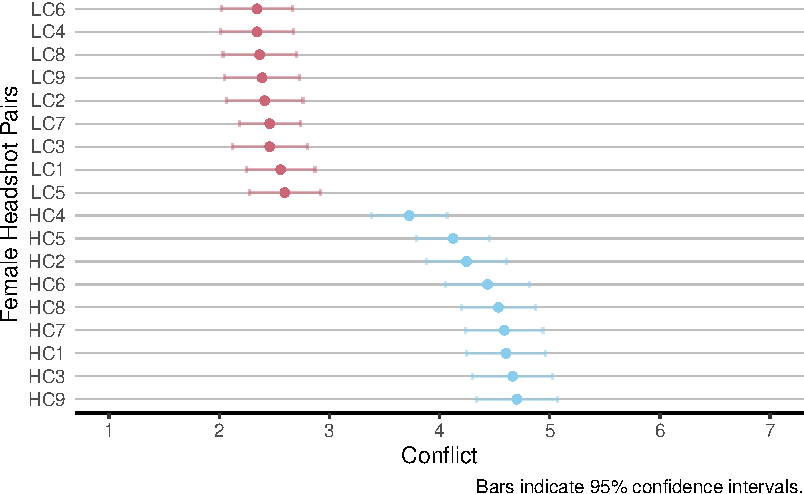
\includegraphics{appendix_sounds_files/figure-pdf/unnamed-chunk-2-1.pdf}

}

\caption{Pre-Test Female Headshots}

}

\end{minipage}%
%
\begin{minipage}[t]{0.50\linewidth}

{\centering 

\raisebox{-\height}{

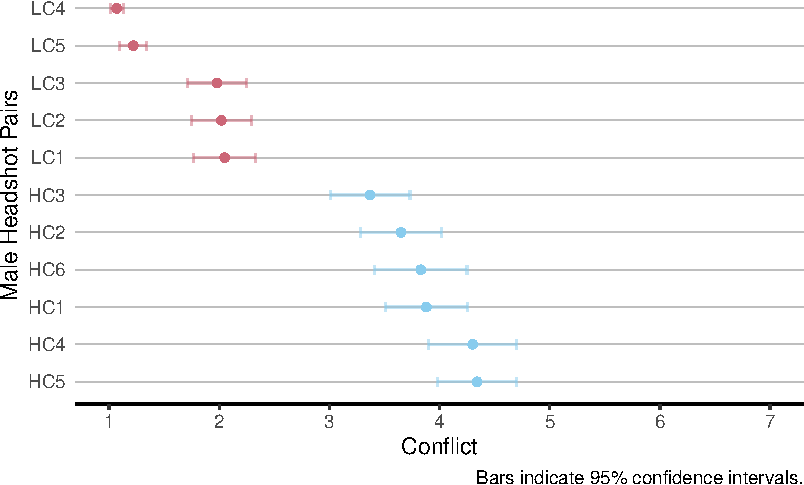
\includegraphics{appendix_sounds_files/figure-pdf/unnamed-chunk-2-2.pdf}

}

\caption{Pre-Test Male Headshots}

}

\end{minipage}%

\end{figure}

The visualizations show on two accounts that the low conflict pairs
(abbreviated with \texttt{LC} and colored in red) are perceived
significantly different than the high conflict (\texttt{HC}, blue)
pairs.

The visualizations also show that there is some variation within these
two conditions. We'll choose the pairs that are the most extreme:
e.g.~we pick the pairs that represent the highest (lowest)
\texttt{conflict} for the \texttt{HC} (\texttt{LC}) condition.

Hence, we implement the pairs listed in the following table. The first
column refers to the codes used in this analysis (displayed in the
visualizations). The second column refers to the gender of the models
shown in each pair and the last columns displays the file names
implemented in oTree.

\begin{longtable}[]{@{}lll@{}}
\toprule\noalign{}
Code & Gender & File Names \\
\midrule\noalign{}
\endhead
\bottomrule\noalign{}
\endlastfoot
HC3 & female & HCP1A, HCP1B \\
HC9 & female & HCP2A, HCP2B \\
HC4 & male & HCP3A, HCP3B \\
HC5 & male & HCP4A, HCP4B \\
LC8 & female & LCP1A, LCP1B \\
LC9 & female & LCP2A, LCP2B \\
LC5 & male & LCP3A, LCP3B \\
LC4 & male & LCP4A, LCP4B \\
\end{longtable}

\hypertarget{sec-sound-stimuli}{%
\section{Stimuli}\label{sec-sound-stimuli}}

All stimuli can be found in our
\href{https://github.com/Howquez/vocalized-preferences/tree/main/software/pilots/preferences/static/models}{Github
repository}.



\end{document}
